\section{PRISMA: Projection of Representations for Interpretability via Sparse Monosemantic Autoencoders}
\label{sec:05_prisma}

\epigraph{
    The purpose of abstraction is not to be vague, but to create a new semantic level in which one can be absolutely precise.
}{Edsger W. Dijkstra}

\newpage

\subsection{Fare luce nella black box degli embedding}
\label{subsec:prisma_intro}
Nel capitolo precedente abbiamo identificato i due ostacoli fondamentali che impediscono di interpretare le rappresentazioni neurali: l'opacità—non conosciamo le direzioni $\mathbf{w}_i$ lungo cui sono codificate le feature—e l'interferenza—anche conoscendole, non potremmo recuperare le intensità $a_i$ in modo pulito a causa della non-ortogonalità. Abbiamo anche delineato una via d'uscita teorica: espandere lo spazio delle rappresentazioni e imporre sparsità, così da forzare ogni feature a occupare un asse dedicato.
\begin{figure}[htbp]
    \centering
    \includegraphics[width=\textwidth]{pictures/cap5/home.png}
    \caption{Home page di PRISMA, l'applicazione sviluppata in questa tesi per la scomposizione degli embedding in feature interpretabili.}
    \label{fig:prisma_home}
\end{figure}
Questo capitolo presenta PRISMA (\textbf{P}rojection of \textbf{R}epresentations for \textbf{I}nterpretability via \textbf{S}parse \textbf{M}onosemantic \textbf{A}utoencoders), un'applicazione sviluppata in questa tesi che implementa concretamente questa strategia. Il nome non è casuale: richiama l'analogia con il prisma ottico, uno strumento che non genera luce, ma la scompone. Quando un fascio di luce bianca attraversa un prisma, ne emergono le componenti spettrali—rosso, arancione, giallo, e così via—che erano già presenti nel fascio originario, ma indistinguibili a occhio nudo. Il prisma non aggiunge informazione: la rende visibile, separando ciò che era mescolato.
\begin{figure}[htbp]
    \centering
    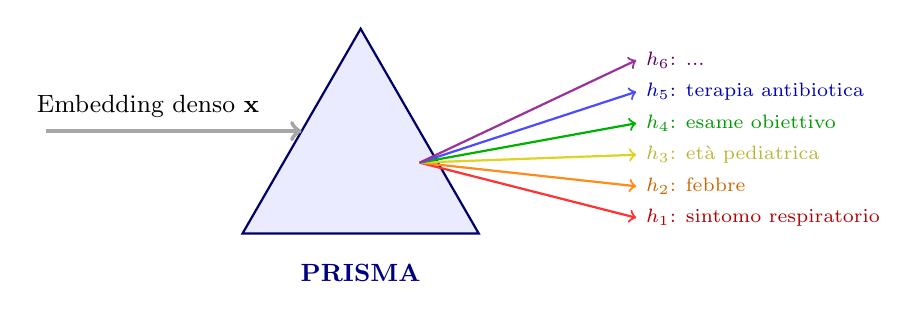
\begin{tikzpicture}[scale=1.0]
        % Prisma (triangolo)
        \coordinate (A) at (0, 0);
        \coordinate (B) at (3, 0);
        \coordinate (C) at (1.5, 2.6);
        
        \fill[blue!8] (A) -- (B) -- (C) -- cycle;
        \draw[thick, blue!40!black] (A) -- (B) -- (C) -- cycle;
        
        % Raggio incidente (bianco/grigio)
        \draw[->, ultra thick, gray!70] (-2.5, 1.3) -- (0.75, 1.3);
        \node[above, font=\small] at (-1.2, 1.35) {Embedding denso $\mathbf{x}$};
        
        % Raggi rifratti (spettro) - escono dal lato destro del prisma
        \draw[->, thick, red!80] (2.25, 0.9) -- (5, 0.2);
        \draw[->, thick, orange!90] (2.25, 0.9) -- (5, 0.6);
        \draw[->, thick, yellow!85!black] (2.25, 0.9) -- (5, 1.0);
        \draw[->, thick, green!70!black] (2.25, 0.9) -- (5, 1.4);
        \draw[->, thick, blue!70] (2.25, 0.9) -- (5, 1.8);
        \draw[->, thick, violet!80] (2.25, 0.9) -- (5, 2.2);
        
        % Etichette feature
        \node[right, font=\scriptsize, red!70!black] at (5, 0.2) {$h_1$: sintomo respiratorio};
        \node[right, font=\scriptsize, orange!80!black] at (5, 0.6) {$h_2$: febbre};
        \node[right, font=\scriptsize, yellow!70!black] at (5, 1.0) {$h_3$: età pediatrica};
        \node[right, font=\scriptsize, green!60!black] at (5, 1.4) {$h_4$: esame obiettivo};
        \node[right, font=\scriptsize, blue!70!black] at (5, 1.8) {$h_5$: terapia antibiotica};
        \node[right, font=\scriptsize, violet!70!black] at (5, 2.2) {$h_6$: ...};
        
        % Etichetta prisma
        \node[font=\small\bfseries, blue!50!black] at (1.5, -0.5) {PRISMA};
        
    \end{tikzpicture}
    \caption{L'analogia ottica di PRISMA. Come un prisma scompone la luce bianca nelle sue componenti spettrali, così PRISMA scompone un embedding denso $\mathbf{x}$ nelle sue feature semantiche costitutive $h_1, h_2, \dots, h_n$. L'informazione era già presente nell'embedding originario, ma codificata in forma opaca; PRISMA la rende esplicita e interpretabile.}
    \label{fig:prisma_analogy}
\end{figure}

PRISMA opera in modo analogo sugli embedding. Un vettore denso $\mathbf{x} \in \mathbb{R}^{768}$, prodotto da un modello come BERT, contiene informazione semantica ricchissima—ma opaca, distribuita su dimensioni che non sappiamo interpretare. PRISMA proietta questo vettore in uno spazio di dimensionalità molto maggiore ($\mathbb{R}^{n}$ con $n \gg 768$), forzando al contempo una rappresentazione sparsa: solo poche componenti $h_i$ possono essere attive per ogni input. Il risultato è una scomposizione in cui ogni componente corrisponde a una feature semantica distinta—un concetto atomico, interpretabile, che possiamo nominare.
L'analogia ha anche una seconda lettura. Il prisma, scomponendo la luce, ci permette di vedere ciò che prima era invisibile. Allo stesso modo, PRISMA fa luce sulla black box degli embedding: non aggiunge capacità predittiva al modello originario, ma rende trasparente ciò che il modello ha appreso. Se la superposition è il meccanismo con cui le reti neurali nascondono la complessità—comprimendo migliaia di concetti in poche centinaia di dimensioni—PRISMA è lo strumento che inverte questo processo, restituendoci una rappresentazione in cui possiamo finalmente leggere quali concetti sono presenti e con quale intensità.
Nel resto di questo capitolo descriveremo l'architettura tecnica che realizza questa scomposizione—lo Sparse Autoencoder—e le metodologie per interpretare automaticamente le feature estratte. Vedremo anche come le feature non siano entità isolate, ma si organizzino in strutture gerarchiche (\textit{feature families}) e come la loro granularità emerga progressivamente all'aumentare della capacità del modello (\textit{feature splitting}).
\subsection{Architettura dello Sparse Autoencoder}
\label{subsec:sae_architecture}

Lo SparseAutoencoder (SAE) è l'architettura neurale al cuore di PRISMA. Come ogni autoencoder, è composto da un encoder che mappa l'input in una rappresentazione latente e un decoder che ricostruisce l'input a partire da essa. La differenza cruciale rispetto agli autoencoder classici—trattati nel Capitolo 2—risiede in due scelte progettuali che invertono la logica tradizionale: lo spazio latente è \textit{overcomplete} anziché compresso, e le attivazioni sono forzate a essere \textit{sparse}.
\subsubsection{Panoramica dell'architettura}
\label{subsubsec:sae_overview}

Seguiamo il formalismo di O'Neill et al.~\parencite{oneill2024disentangling}. Sia $\mathbf{x} \in \mathbb{R}^d$ l'embedding di input (ad esempio, il vettore a 768 dimensioni prodotto da BERT) e $\mathbf{h} \in \mathbb{R}^n$ la rappresentazione latente, con $n > d$. L'architettura è definita da due insiemi di parametri apprendibili:
\begin{equation}
    \theta = \{W_e, \mathbf{b}_e\}, \qquad \phi = \{W_d, \mathbf{b}_d\}
\end{equation}
che parametrizzano rispettivamente l'encoder e il decoder.
L'\textbf{encoder} $f_\theta$ mappa l'input nella rappresentazione latente:
\begin{equation}
    \mathbf{h} = f_\theta(\mathbf{x}) = \sigma(W_e \mathbf{x} + \mathbf{b}_e)
    \label{eq:sae_encoder}
\end{equation}
dove $W_e \in \mathbb{R}^{n \times d}$ è la matrice dei pesi, $\mathbf{b}_e \in \mathbb{R}^n$ è il vettore di bias, e $\sigma(\cdot)$ è una funzione di attivazione non lineare (tipicamente ReLU).
Il \textbf{decoder} $g_\phi$ ricostruisce l'input dalla rappresentazione latente:
\begin{equation}
    \hat{\mathbf{x}} = g_\phi(\mathbf{h}) = W_d \mathbf{h} + \mathbf{b}_d
    \label{eq:sae_decoder}
\end{equation}
dove $W_d \in \mathbb{R}^{d \times n}$ è la matrice dei pesi e $\mathbf{b}_d \in \mathbb{R}^d$ è il vettore di bias.
La Figura~\ref{fig:sae_architecture} illustra il flusso dei dati attraverso l'architettura. Si noti immediatamente l'asimmetria nelle dimensioni: l'input $\mathbf{x}$ ha $d$ componenti, mentre la rappresentazione latente $\mathbf{h}$ ne ha $n \gg d$. Questa espansione—l'opposto della compressione tipica degli autoencoder—è la prima chiave per ottenere il disentanglement. La seconda chiave, visibile nei pochi cerchi verdi tra i molti grigi, è la sparsità: per ogni input, solo una piccola frazione delle $n$ componenti di $\mathbf{h}$ è diversa da zero.
\begin{figure}[htbp]
    \centering
    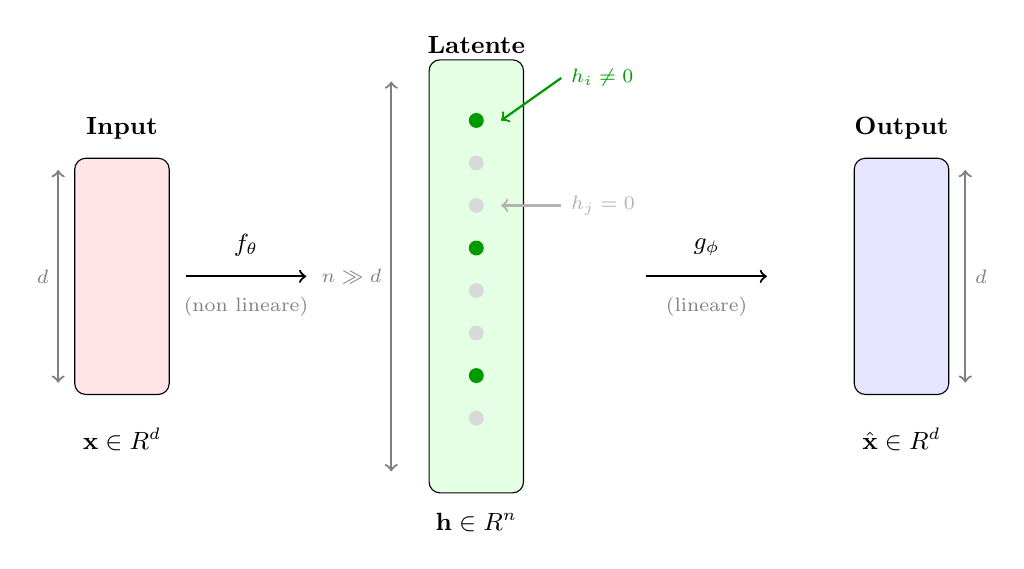
\begin{tikzpicture}[scale=0.9]
        % Input
        \node[draw, rectangle, minimum width=1.2cm, minimum height=3cm, fill=red!10, rounded corners] (input) at (0, 0) {};
        \node[below, font=\small] at (0, -2.0) {$\mathbf{x} \in \mathbb{R}^d$};
        \node[above, font=\small\bfseries] at (0, 1.8) {Input};
        
        % Encoder arrow
        \draw[->, thick] (0.9, 0) -- (2.6, 0);
        \node[above, font=\small] at (1.75, 0.15) {$f_\theta$};
        \node[below, font=\scriptsize, gray] at (1.75, -0.15) {(non lineare)};
        
        % Latent space (overcomplete)
        \node[draw, rectangle, minimum width=1.2cm, minimum height=5.5cm, fill=green!10, rounded corners] (latent) at (5, 0) {};
        \node[below, font=\small] at (5, -3.2) {$\mathbf{h} \in \mathbb{R}^n$};
        \node[above, font=\small\bfseries] at (5, 3.0) {Latente};
        
        % Sparse activations (dots)
        \fill[green!60!black] (5, 2.2) circle (3pt);
        \fill[gray!30] (5, 1.6) circle (3pt);
        \fill[gray!30] (5, 1.0) circle (3pt);
        \fill[green!60!black] (5, 0.4) circle (3pt);
        \fill[gray!30] (5, -0.2) circle (3pt);
        \fill[gray!30] (5, -0.8) circle (3pt);
        \fill[green!60!black] (5, -1.4) circle (3pt);
        \fill[gray!30] (5, -2.0) circle (3pt);
        
        % Annotation for sparsity
        \draw[<-, thick, green!60!black] (5.35, 2.2) -- (6.2, 2.8);
        \node[right, font=\scriptsize, green!60!black, align=left] at (6.2, 2.8) {$h_i \neq 0$};
        
        \draw[<-, thick, gray!60] (5.35, 1.0) -- (6.2, 1.0);
        \node[right, font=\scriptsize, gray!60, align=left] at (6.2, 1.0) {$h_j = 0$};
        
        % Decoder arrow
        \draw[->, thick] (7.4, 0) -- (9.1, 0);
        \node[above, font=\small] at (8.25, 0.15) {$g_\phi$};
        \node[below, font=\scriptsize, gray] at (8.25, -0.15) {(lineare)};
        
        % Output
        \node[draw, rectangle, minimum width=1.2cm, minimum height=3cm, fill=blue!10, rounded corners] (output) at (11, 0) {};
        \node[below, font=\small] at (11, -2.0) {$\hat{\mathbf{x}} \in \mathbb{R}^d$};
        \node[above, font=\small\bfseries] at (11, 1.8) {Output};
        
        % Dimension annotations
        \draw[<->, thick, gray] (-0.9, -1.5) -- (-0.9, 1.5);
        \node[left, font=\scriptsize, gray] at (-0.9, 0) {$d$};
        
        \draw[<->, thick, gray] (3.8, -2.75) -- (3.8, 2.75);
        \node[left, font=\scriptsize, gray] at (3.8, 0) {$n \gg d$};
        
        \draw[<->, thick, gray] (11.9, -1.5) -- (11.9, 1.5);
        \node[right, font=\scriptsize, gray] at (11.9, 0) {$d$};
        
    \end{tikzpicture}
    \caption{Architettura dello Sparse Autoencoder. L'encoder $f_\theta$ (non lineare) mappa l'input $\mathbf{x}$ in uno spazio latente \textit{overcomplete} di dimensione $n \gg d$. La sparsità forza solo poche componenti di $\mathbf{h}$ (cerchi verdi) ad essere attive, mentre le altre (cerchi grigi) restano nulle. Il decoder $g_\phi$ (lineare) ricostruisce l'input come combinazione delle sole direzioni attive.}
    \label{fig:sae_architecture}
\end{figure}
Un'asimmetria meno evidente, ma altrettanto importante, riguarda la natura delle due trasformazioni: l'encoder è non lineare (Equazione~\ref{eq:sae_encoder}), mentre il decoder è lineare (Equazione~\ref{eq:sae_decoder}). Questa scelta non è arbitraria: come vedremo nelle prossime sezioni, è precisamente la linearità del decoder a garantire che le feature estratte siano interpretabili come direzioni nello spazio degli embedding—la condizione necessaria per ottenere il disentanglement discusso nel Capitolo~\ref{sec:04_disentangling_dense_embeddings_with_sparse_autoencoders}.
subsubsection{L'encoder: una proiezione non lineare}
\label{subsubsec:sae_encoder}

L'encoder ha il compito di analizzare l'embedding in ingresso e determinare quali feature sono presenti e con quale intensità. Riprendendo l'Equazione~\ref{eq:sae_encoder}:
\begin{equation}
    \mathbf{h} = f_\theta(\mathbf{x}) = \sigma(W_e \mathbf{x} + \mathbf{b}_e)
\end{equation}
questa trasformazione si compone di due passaggi: una proiezione lineare $W_e \mathbf{x} + \mathbf{b}_e$ seguita da una non linearità $\sigma(\cdot)$.
La matrice $W_e \in \mathbb{R}^{n \times d}$ ha $n$ righe, una per ogni componente dello spazio latente. Indichiamo con $\mathbf{e}_i^T$ la $i$-esima riga: è un vettore in $\mathbb{R}^d$ che vive nello stesso spazio dell'input $\mathbf{x}$. La proiezione lineare calcola, per ogni feature $i$, un punteggio grezzo:
\begin{equation}
    z_i = \mathbf{e}_i^T \mathbf{x} + b_{e,i}
\end{equation}
Questo punteggio misura quanto l'input $\mathbf{x}$ sia allineato con la direzione $\mathbf{e}_i$: se i due vettori puntano in direzioni simili, il prodotto scalare sarà elevato; se puntano in direzioni opposte, sarà negativo.
La non linearità $\sigma(\cdot)$—tipicamente la funzione ReLU—trasforma i punteggi grezzi nelle attivazioni finali:
\begin{equation}
    h_i = \sigma(z_i) = \max(0, z_i)
\end{equation}
La scelta della ReLU serve a due scopi. Il primo è garantire attivazioni non negative: una feature è ``presente'' con una certa intensità positiva, oppure è ``assente'' (attivazione nulla). Non avrebbe senso, dal punto di vista interpretativo, che una feature fosse presente con intensità negativa. Il secondo scopo è indurre sparsità naturale: la ReLU azzera tutte le pre-attivazioni negative, contribuendo alla sparsità della rappresentazione anche prima di applicare vincoli espliciti come il Top-K che vedremo nella Sezione~\ref{subsec:loss_function}.
\begin{figure}[htbp]
    \centering
    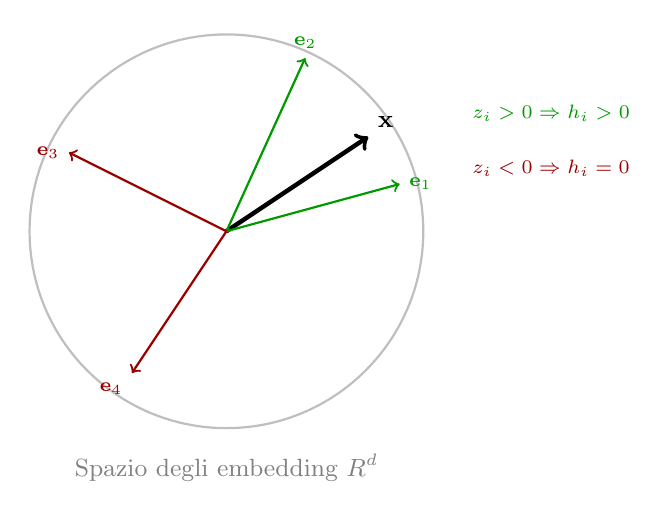
\begin{tikzpicture}[scale=1.0]
        % Spazio embedding (cerchio)
        \draw[thick, gray!50] (0,0) circle (2.5cm);
        \node[font=\small, gray] at (0, -3.0) {Spazio degli embedding $\mathbb{R}^d$};
        
        % Vettore input x
        \draw[->, ultra thick, black] (0,0) -- (1.8, 1.2);
        \node[above right, font=\small\bfseries] at (1.8, 1.2) {$\mathbf{x}$};
        
        % Direzioni di rilevamento encoder
        \draw[->, thick, green!60!black] (0,0) -- (2.2, 0.6);
        \node[right, font=\scriptsize, green!60!black] at (2.2, 0.6) {$\mathbf{e}_1$};
        
        \draw[->, thick, green!60!black] (0,0) -- (1.0, 2.2);
        \node[above, font=\scriptsize, green!60!black] at (1.0, 2.2) {$\mathbf{e}_2$};
        
        \draw[->, thick, red!60!black] (0,0) -- (-2.0, 1.0);
        \node[left, font=\scriptsize, red!60!black] at (-2.0, 1.0) {$\mathbf{e}_3$};
        
        \draw[->, thick, red!60!black] (0,0) -- (-1.2, -1.8);
        \node[below left, font=\scriptsize, red!60!black] at (-1.2, -1.8) {$\mathbf{e}_4$};
        
        % Legenda
        \node[right, font=\scriptsize, green!60!black] at (3.0, 1.5) {$z_i > 0 \Rightarrow h_i > 0$};
        \node[right, font=\scriptsize, red!60!black] at (3.0, 0.8) {$z_i < 0 \Rightarrow h_i = 0$};
        
    \end{tikzpicture}
    \caption{L'encoder come rilevatore di feature. L'input $\mathbf{x}$ viene proiettato sulle direzioni $\mathbf{e}_i$ (righe di $W_e$). Le direzioni sufficientemente allineate con $\mathbf{x}$ (in verde) producono pre-attivazioni positive $z_i > 0$, che la ReLU preserva; quelle non allineate (in rosso) producono $z_i < 0$ e vengono azzerate.}
    \label{fig:encoder_detection}
\end{figure}

È importante chiarire il ruolo di questi vettori $\mathbf{e}_i$. Essi non coincidono con le direzioni $\mathbf{w}_i$ introdotte nel Capitolo~\ref{sec:04_disentangling_dense_embeddings_with_sparse_autoencoders}: le $\mathbf{w}_i$ sono le direzioni lungo cui le feature sono \textit{codificate} nello spazio degli embedding, e corrispondono—come vedremo—alle colonne della matrice del decoder $W_d$. Le $\mathbf{e}_i$, invece, sono direzioni ausiliarie che l'encoder utilizza per \textit{rilevare} le feature nell'input. In uno scenario ideale con feature perfettamente ortogonali, le due coinciderebbero: per rilevare una feature basterebbe proiettare lungo la sua stessa direzione. Ma nella superposition le $\mathbf{w}_i$ non sono ortogonali, e proiettare direttamente lungo di esse causerebbe l'interferenza descritta nel capitolo precedente. L'encoder impara quindi direzioni $\mathbf{e}_i \neq \mathbf{w}_i$ che compensano questa sovrapposizione.

Dal punto di vista dell'interpretabilità, le $\mathbf{e}_i$ non hanno un significato semantico diretto: sono un meccanismo interno che serve all'encoder per svolgere il suo compito. Ciò che ci interessa—e che costituisce il vero output interpretabile del SAE—sono le attivazioni $h_i$ e le direzioni $\mathbf{w}_i$ del decoder. La corrispondenza è uno-a-uno: per ogni $i \in \{1, \dots, n\}$, il vettore $\mathbf{e}_i$ rileva la feature $i$ producendo l'attivazione $h_i$, che a sua volta pesa la direzione $\mathbf{w}_i$ nella ricostruzione. Ma mentre $\mathbf{e}_i$ è un dettaglio implementativo, $\mathbf{w}_i$ rappresenta la feature stessa nello spazio semantico.

La non linearità dell'encoder è dunque essenziale: permette di implementare una logica di rilevamento sofisticata in presenza di sovrapposizione. Il decoder, come vedremo, ha un compito diverso—ricostruire l'input come combinazione di feature—e per quel compito la linearità non è solo possibile, ma necessaria.

\subsubsection{Lo spazio latente overcomplete}
\label{subsubsec:sae_overcomplete}

Nel Capitolo~\ref{sec:04_disentangling_dense_embeddings_with_sparse_autoencoders} abbiamo identificato il paradosso della capacità: un modello come BERT rappresenta decine di migliaia di concetti con soli 768 neuroni. La superposition risolve questo problema comprimendo le feature come direzioni oblique, ma al costo dell'opacità e dell'interferenza. Se vogliamo invertire questo processo—ottenere una rappresentazione in cui ogni feature abbia un asse dedicato—servono più dimensioni di quelle originarie.

Questa è l'intuizione alla base dello spazio latente \textit{overcomplete}. A differenza degli autoencoder classici, che comprimono l'input in un bottleneck di dimensionalità inferiore ($n < d$), lo Sparse Autoencoder espande la rappresentazione in uno spazio più grande:
\begin{equation}
    n > d
\end{equation}
dove $d$ è la dimensionalità dell'embedding originale e $n$ è la dimensionalità dello spazio latente.

Il rapporto tra queste due quantità è detto \textit{expansion factor}:
\begin{equation}
    \rho = \frac{n}{d}
\end{equation}
e assume tipicamente valori compresi tra 2 e 9~\parencite{oneill2024disentangling}. Un expansion factor $\rho = 4$, ad esempio, significa che lo spazio latente ha quattro volte le dimensioni dell'input: per un embedding BERT a 768 dimensioni, lo spazio latente avrebbe $n = 3072$ componenti.
\begin{figure}[htbp]
    \centering
    \begin{tikzpicture}[scale=0.6, transform shape, node distance=1cm]
        % Nodes
        \node[draw, rectangle, minimum height=3cm, minimum width=0.5cm, fill=gray!20] (input) at (0,0) {$\mathbf{x} \in \mathbb{R}^{d}$};
        \node[draw, trapezium, trapezium angle=70, shape border rotate=270, minimum height=1.5cm, fill=orange!15] (enc) at (2.5,0) {Encoder};
        \node[draw, rectangle, minimum height=1.2cm, minimum width=0.5cm, fill=orange!30] (latent) at (5,0) {$\mathbf{z} \in \mathbb{R}^{m}$};
        \node at (5, -1.5) {\footnotesize $m < d$};
        \node[draw, trapezium, trapezium angle=70, shape border rotate=90, minimum height=1.5cm, fill=orange!15] (dec) at (7.5,0) {Decoder};
        \node[draw, rectangle, minimum height=3cm, minimum width=0.5cm, fill=gray!20] (output) at (10,0) {$\hat{\mathbf{x}} \in \mathbb{R}^{d}$};
        % Arrows
        \draw[->, thick] (input) -- (enc);
        \draw[->, thick] (enc) -- (latent);
        \draw[->, thick] (latent) -- (dec);
        \draw[->, thick] (dec) -- (output);
    \end{tikzpicture}
    \caption{Autoencoder classico: il bottleneck forza la compressione informativa ($m < d$).}
    \label{fig:ae_classico}
\end{figure}

\begin{figure}[htbp]
    \centering
    \begin{tikzpicture}[scale=0.6, transform shape, node distance=1cm]
        % Nodes
        \node[draw, rectangle, minimum height=2cm, minimum width=0.5cm, fill=gray!20] (input) at (0,0) {$\mathbf{x} \in \mathbb{R}^{d}$};
        
        % Trapezium for Expansion
        \node[draw, trapezium, trapezium angle=70, shape border rotate=90, minimum height=1.5cm, fill=green!15] (enc) at (2.5,0) {Encoder};
        
        % Sparse Latent
        \node[draw, rectangle, minimum height=4cm, minimum width=0.5cm, fill=green!30, label=above:spazio latente $\mathbf{h}$] (latent) at (5,0) {$\mathbf{h} \in \mathbb{R}^{n}$};
        \node at (5, -2.8) {\footnotesize $n > d$};
        
        % Trapezium for Compression
        \node[draw, trapezium, trapezium angle=70, shape border rotate=270, minimum height=1.5cm, fill=green!15] (dec) at (7.5,0) {Decoder};
        
        \node[draw, rectangle, minimum height=2cm, minimum width=0.5cm, fill=gray!20] (output) at (10,0) {$\hat{\mathbf{x}} \in \mathbb{R}^{d}$};
        % Arrows
        \draw[->, thick] (input) -- (enc);
        \draw[->, thick] (enc) -- (latent);
        \draw[->, thick] (latent) -- (dec);
        \draw[->, thick] (dec) -- (output);
    \end{tikzpicture}
    \caption{Sparse Autoencoder: lo spazio latente è overcomplete ($n > d$), con abbastanza dimensioni affinché ogni feature possa avere un asse dedicato.}
    \label{fig:sae_overcomplete}
\end{figure}
La scelta di $\rho$ riflette un compromesso. Valori troppo bassi potrebbero non fornire abbastanza dimensioni per rappresentare tutte le feature del modello originario: se BERT codifica 50.000 concetti in 768 dimensioni, un expansion factor $\rho = 2$ fornirebbe solo 1.536 assi—ancora insufficienti per il disentanglement completo. Valori troppo alti, d'altra parte, aumentano il costo computazionale e il rischio di overfitting: con troppe dimensioni disponibili, il modello potrebbe apprendere feature spurie o ridondanti.
Nella pratica, la scelta dell'expansion factor dipende dal dominio e dalla granularità desiderata. O'Neill et al.~\parencite{oneill2024disentangling} osservano che, per embedding di articoli scientifici, valori di $\rho$ tra 2 e 6 producono feature interpretabili con un buon compromesso tra capacità e qualità. Expansion factor maggiori tendono a produrre feature più specifiche e granulari—un fenomeno che esploreremo nella Sezione~\ref{subsec:feature_splitting} sotto il nome di \textit{feature splitting}.
È importante sottolineare che l'overcompletezza, da sola, non garantisce il disentanglement. Uno spazio con $n > d$ dimensioni offre la \textit{possibilità} che ogni feature abbia un asse dedicato, ma nulla impedisce al modello di utilizzare questo spazio in modo ridondante o non interpretabile. È il vincolo di sparsità—che vedremo nella Sezione~\ref{subsec:loss_function}—a forzare il modello a sfruttare l'overcompletezza nel modo desiderato: poche attivazioni per input, ciascuna corrispondente a una feature distinta.

\subsubsection{La linearità del decoder: la chiave del disentanglement}
\label{subsubsec:sae_decoder_linearity}

Abbiamo visto che l'encoder è una funzione non lineare: la ReLU introduce una soglia che azzera le attivazioni negative, permettendo di rilevare le feature in modo selettivo. Il decoder, al contrario, è una trasformazione puramente lineare. Riprendendo l'Equazione~\ref{eq:sae_decoder}:
\begin{equation}
    \hat{\mathbf{x}} = g_\phi(\mathbf{h}) = W_d \mathbf{h} + \mathbf{b}_d
\end{equation}
Questa asimmetria non è un dettaglio implementativo: è la scelta architetturale che rende possibile il disentanglement.

Per capire perché, espandiamo il prodotto matrice-vettore $W_d \mathbf{h}$. La matrice $W_d \in \mathbb{R}^{d \times n}$ ha $n$ colonne; indichiamo la $i$-esima colonna con $\mathbf{w}_i \in \mathbb{R}^d$. Il vettore $\mathbf{h} \in \mathbb{R}^n$ ha $n$ componenti $h_1, h_2, \dots, h_n$. Il prodotto può essere scritto come:
\begin{equation}
    W_d \mathbf{h} = \sum_{i=1}^{n} h_i \cdot \mathbf{w}_i
    \label{eq:decoder_linear_combination}
\end{equation}
La ricostruzione completa diventa quindi:
\begin{equation}
    \hat{\mathbf{x}} = \sum_{i=1}^{n} h_i \cdot \mathbf{w}_i + \mathbf{b}_d
    \label{eq:reconstruction_explicit}
\end{equation}

Questa equazione è il cuore dell'interpretabilità dello Sparse Autoencoder. La ricostruzione $\hat{\mathbf{x}}$ è una \textit{combinazione lineare} dei vettori $\mathbf{w}_i$, pesata dalle attivazioni $h_i$. Ogni vettore $\mathbf{w}_i$ rappresenta il contributo che la feature $i$ apporta alla ricostruzione quando è attiva con intensità unitaria. L'attivazione $h_i$ modula questo contributo: se $h_i = 0$ la feature non contribuisce; se $h_i > 0$, il vettore $\mathbf{w}_i$ viene sommato alla ricostruzione con peso proporzionale all'intensità della feature.

I vettori $\mathbf{w}_i$ sono esattamente le direzioni delle feature di cui abbiamo parlato nel Capitolo~\ref{sec:04_disentangling_dense_embeddings_with_sparse_autoencoders}. Là avevamo scritto l'embedding come combinazione di direzioni sconosciute:
\begin{equation}
    \mathbf{x} = \sum_i a_i \, \mathbf{w}_i
\end{equation}
lamentando di non conoscere né le direzioni $\mathbf{w}_i$ né le intensità $a_i$. Lo Sparse Autoencoder risolve entrambi i problemi: le direzioni $\mathbf{w}_i$ sono le colonne della matrice $W_d$, apprese durante l'addestramento e quindi note; le intensità $a_i$ corrispondono alle attivazioni $h_i$, calcolate dall'encoder per ogni input.

\begin{notebox}
\textbf{La chiave del disentanglement}\\

Nel Capitolo~\ref{sec:04_disentangling_dense_embeddings_with_sparse_autoencoders} abbiamo identificato due problemi della superposition:
\begin{enumerate}
    \item \textbf{Opacità}: non conosciamo le direzioni $\mathbf{w}_i$ delle feature
    \item \textbf{Interferenza}: non possiamo recuperare le intensità $a_i$ a causa della non-ortogonalità
\end{enumerate}
Lo Sparse Autoencoder affronta entrambi:
\begin{enumerate}
    \item Le direzioni $\mathbf{w}_i$ sono le colonne di $W_d$, apprese e ispezionabili
    \item Le intensità $h_i$ sono calcolate dall'encoder, che impara a compensare l'interferenza
\end{enumerate}
\end{notebox}

È istruttivo confrontare questa situazione con un decoder non lineare. Supponiamo di aggiungere una ReLU anche al decoder:
\begin{equation}
    \hat{\mathbf{x}} = \sigma(W_d \mathbf{h} + \mathbf{b}_d)
\end{equation}
In questo caso la ricostruzione non sarebbe più una combinazione lineare delle colonne di $W_d$. Le interazioni tra feature diventerebbero opache: il contributo della feature $i$ alla ricostruzione dipenderebbe non solo da $h_i$ e $\mathbf{w}_i$, ma anche da tutte le altre attivazioni e dalla soglia della ReLU. Perderemmo la possibilità di dire ``questa componente della ricostruzione viene dalla feature $i$''.

La linearità del decoder garantisce invece una proprietà fondamentale: \textit{additività dei contributi}. Se due feature $i$ e $j$ sono attive, i loro contributi alla ricostruzione sono semplicemente sommati:
\begin{equation}
    \hat{\mathbf{x}} = h_i \cdot \mathbf{w}_i + h_j \cdot \mathbf{w}_j + \sum_{k \neq i,j} h_k \cdot \mathbf{w}_k + \mathbf{b}_d
\end{equation}
Non c'è interazione nascosta tra $\mathbf{w}_i$ e $\mathbf{w}_j$: ciascuna feature contribuisce in modo indipendente e trasparente. Questa trasparenza è ciò che rende le feature interpretabili.

\begin{figure}[htbp]
    \centering
    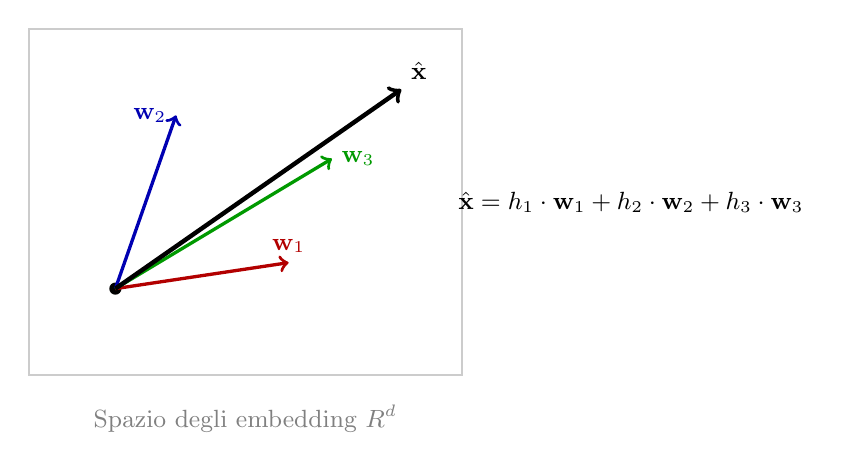
\begin{tikzpicture}[scale=1.1]
        % Spazio embedding
        \draw[thick, gray!40] (-0.5,-0.5) -- (4.5,-0.5) -- (4.5,3.5) -- (-0.5,3.5) -- cycle;
        \node[font=\small, gray] at (2, -1.0) {Spazio degli embedding $\mathbb{R}^d$};
        
        % Origine
        \fill[black] (0.5, 0.5) circle (2pt);
        
        % Vettori w_i (colonne del decoder)
        \draw[->, very thick, red!70!black] (0.5, 0.5) -- (2.5, 0.8);
        \node[above, font=\small, red!70!black] at (2.5, 0.8) {$\mathbf{w}_1$};
        
        \draw[->, very thick, blue!70!black] (0.5, 0.5) -- (1.2, 2.5);
        \node[left, font=\small, blue!70!black] at (1.2, 2.5) {$\mathbf{w}_2$};
        
        \draw[->, very thick, green!60!black] (0.5, 0.5) -- (3.0, 2.0);
        \node[right, font=\small, green!60!black] at (3.0, 2.0) {$\mathbf{w}_3$};
        
        % Vettore ricostruito (combinazione)
        \draw[->, ultra thick, black] (0.5, 0.5) -- (3.8, 2.8);
        \node[above right, font=\small\bfseries] at (3.8, 2.8) {$\hat{\mathbf{x}}$};
        
        % Equazione
        \node[font=\small, align=left] at (6.5, 1.5) {
            $\hat{\mathbf{x}} = h_1 \cdot \mathbf{w}_1 + h_2 \cdot \mathbf{w}_2 + h_3 \cdot \mathbf{w}_3$
        };
        
    \end{tikzpicture}
    \caption{La ricostruzione come combinazione lineare. Ogni colonna $\mathbf{w}_i$ della matrice del decoder rappresenta una direzione nello spazio degli embedding. La ricostruzione $\hat{\mathbf{x}}$ è la somma dei vettori $\mathbf{w}_i$ pesati dalle rispettive attivazioni $h_i$. La linearità garantisce che ogni feature contribuisca in modo indipendente e trasparente.}
    \label{fig:decoder_linear_combination}
\end{figure}

La linearità ha anche un'altra conseguenza importante: ogni colonna $\mathbf{w}_i$ può essere studiata in isolamento. Possiamo chiederci: ``quale direzione nello spazio degli embedding rappresenta la feature $i$?'' e rispondere ispezionando direttamente $\mathbf{w}_i$. Possiamo calcolare la similarità tra due feature confrontando $\mathbf{w}_i$ e $\mathbf{w}_j$. Possiamo persino intervenire sulla rappresentazione, aumentando o diminuendo un'attivazione $h_i$ per ``aggiungere'' o ``rimuovere'' una feature dalla ricostruzione. Nulla di tutto questo sarebbe possibile con un decoder non lineare.

\subsubsection{Feature come direzioni nello spazio degli embedding}
\label{subsubsec:features_as_directions}

Abbiamo stabilito che le colonne $\mathbf{w}_i$ della matrice del decoder rappresentano le feature apprese dal modello. Ma cosa significa, concretamente, che una feature è una ``direzione nello spazio degli embedding''?

Consideriamo lo spazio $\mathbb{R}^d$ in cui vivono gli embedding—ad esempio, lo spazio a 768 dimensioni di BERT. Ogni punto di questo spazio corrisponde a un possibile embedding, cioè alla rappresentazione di un testo. Punti vicini rappresentano testi semanticamente simili; punti lontani rappresentano testi dissimili. In questo spazio, una direzione non è semplicemente un punto, ma un \textit{asse lungo cui spostarsi}.

Ogni colonna $\mathbf{w}_i \in \mathbb{R}^d$ definisce una di queste direzioni. Muoversi lungo $\mathbf{w}_i$, partendo da un embedding $\mathbf{x}$, significa aggiungere o intensificare un certo aspetto semantico. Se $\mathbf{w}_{42}$ rappresenta il concetto di ``febbre'', allora:
\begin{equation}
    \mathbf{x}' = \mathbf{x} + \alpha \cdot \mathbf{w}_{42}
\end{equation}
produce un embedding $\mathbf{x}'$ in cui il concetto di febbre è più presente rispetto a $\mathbf{x}$. Il parametro $\alpha > 0$ controlla l'intensità di questa aggiunta. Questa è esattamente l'operazione che il decoder compie implicitamente: ricostruisce l'embedding sommando le direzioni delle feature attive, ciascuna pesata dalla propria attivazione.

Durante l'addestramento, le colonne di $W_d$ vengono tipicamente normalizzate a norma unitaria:
\begin{equation}
    \|\mathbf{w}_i\| = 1 \quad \forall i \in \{1, \dots, n\}
\end{equation}
Questa normalizzazione ha due scopi. Il primo è separare il ruolo della direzione da quello dell'intensità: $\mathbf{w}_i$ specifica \textit{quale} concetto, mentre $h_i$ specifica \textit{quanto} di quel concetto è presente. Senza normalizzazione, la stessa informazione potrebbe essere codificata sia nella norma di $\mathbf{w}_i$ che nel valore di $h_i$, creando ambiguità. Il secondo scopo è stabilizzare l'addestramento, evitando che alcune colonne crescano arbitrariamente a scapito di altre.

\begin{figure}[htbp]
    \centering
    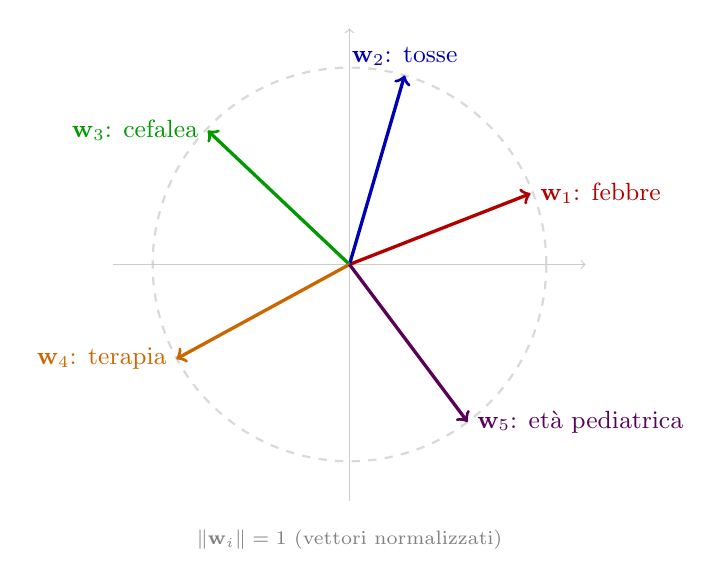
\begin{tikzpicture}[scale=1.0]
        % Cerchio unitario (per suggerire normalizzazione)
        \draw[thick, gray!30, dashed] (0,0) circle (2.5cm);
        
        % Assi di riferimento (grigi, sottili)
        \draw[gray!40, ->] (-3, 0) -- (3, 0);
        \draw[gray!40, ->] (0, -3) -- (0, 3);
        
        % Feature directions (normalizzate, sulla circonferenza)
        \draw[->, very thick, red!70!black] (0,0) -- (2.3, 0.9);
        \node[right, font=\small, red!70!black] at (2.3, 0.9) {$\mathbf{w}_1$: febbre};
        
        \draw[->, very thick, blue!70!black] (0,0) -- (0.7, 2.4);
        \node[above, font=\small, blue!70!black] at (0.7, 2.4) {$\mathbf{w}_2$: tosse};
        
        \draw[->, very thick, green!60!black] (0,0) -- (-1.8, 1.7);
        \node[left, font=\small, green!60!black] at (-1.8, 1.7) {$\mathbf{w}_3$: cefalea};
        
        \draw[->, very thick, orange!80!black] (0,0) -- (-2.2, -1.2);
        \node[left, font=\small, orange!80!black] at (-2.2, -1.2) {$\mathbf{w}_4$: terapia};
        
        \draw[->, very thick, violet!70!black] (0,0) -- (1.5, -2.0);
        \node[right, font=\small, violet!70!black] at (1.5, -2.0) {$\mathbf{w}_5$: età pediatrica};
        
        % Nota sulla normalizzazione
        \node[font=\scriptsize, gray] at (0, -3.5) {$\|\mathbf{w}_i\| = 1$ (vettori normalizzati)};
        
    \end{tikzpicture}
    \caption{Feature come direzioni normalizzate nello spazio degli embedding. Ogni colonna $\mathbf{w}_i$ del decoder definisce una direzione unitaria associata a un concetto semantico. Le direzioni non sono ortogonali: feature semanticamente correlate (come febbre e tosse) possono puntare in direzioni simili.}
    \label{fig:features_as_directions}
\end{figure}

È importante osservare che le direzioni $\mathbf{w}_i$ non sono, in generale, ortogonali tra loro. Questo potrebbe sembrare un fallimento: nel Capitolo~\ref{sec:04_disentangling_dense_embeddings_with_sparse_autoencoders} abbiamo presentato l'ortogonalità come condizione ideale per il disentanglement. Ma l'ortogonalità perfetta è impossibile quando il numero di feature $n$ supera la dimensionalità dello spazio $d$: in $\mathbb{R}^d$ possono esistere al massimo $d$ vettori mutuamente ortogonali. Con $n = 3072$ feature e $d = 768$ dimensioni, la non-ortogonalità è una necessità matematica.

Ciò che lo Sparse Autoencoder garantisce non è l'ortogonalità delle direzioni, ma la loro \textit{esplicitezza}. A differenza della superposition originaria—dove le direzioni erano sconosciute e mescolate—qui ogni $\mathbf{w}_i$ è un vettore ispezionabile, memorizzato come colonna della matrice $W_d$. Possiamo misurare il prodotto scalare $\mathbf{w}_i^T \mathbf{w}_j$ per quantificare la sovrapposizione tra due feature. Possiamo visualizzare le direzioni, confrontarle, raggrupparle. L'interferenza geometrica non è eliminata, ma è resa trasparente.

Questa trasparenza apre la strada all'interpretazione. Se $\mathbf{w}_i$ è una direzione nello spazio degli embedding, possiamo chiederci: quali testi producono embedding allineati con questa direzione? Ovvero: per quali input l'attivazione $h_i$ è elevata? La risposta a questa domanda—trovare i testi che ``accendono'' una feature—è il primo passo per assegnare un significato semantico alle direzioni apprese. Vedremo nella Sezione~\ref{subsec:interpretability} come questo processo possa essere automatizzato utilizzando un modello linguistico come interprete.

\begin{notebox}
\textbf{Riepilogo: l'architettura dello Sparse Autoencoder}\\
Lo Sparse Autoencoder trasforma un embedding denso $\mathbf{x} \in \mathbb{R}^d$ in una rappresentazione sparsa $\mathbf{h} \in \mathbb{R}^n$ con $n > d$:
\begin{itemize}
    \item L'\textbf{encoder} (non lineare) rileva quali feature sono presenti, producendo attivazioni $h_i \geq 0$
    \item Lo \textbf{spazio latente} è overcomplete: abbastanza dimensioni per rappresentare molte feature
    \item Il \textbf{decoder} (lineare) ricostruisce l'input come $\hat{\mathbf{x}} = \sum_i h_i \mathbf{w}_i + \mathbf{b}_d$
    \item Le \textbf{colonne} $\mathbf{w}_i$ di $W_d$ sono le direzioni delle feature, ispezionabili e interpretabili
\end{itemize}
La linearità del decoder è la chiave: garantisce che ogni feature contribuisca in modo indipendente e trasparente alla ricostruzione.
\end{notebox}

\subsection{Funzione di perdita e addestramento}
\label{subsec:loss_function}

L'architettura dello Sparse Autoencoder—encoder non lineare, spazio overcomplete, decoder lineare—definisce la struttura del modello. Ma è la funzione di perdita a determinare \textit{cosa} il modello apprende. In questa sezione esaminiamo i tre componenti della loss function e il loro ruolo nel produrre rappresentazioni sparse e interpretabili.

\subsubsection{La funzione di perdita complessiva}
\label{subsubsec:loss_overview}

L'obiettivo dell'addestramento è duplice: il modello deve ricostruire fedelmente gli embedding originali, ma deve farlo utilizzando rappresentazioni sparse. Questi due obiettivi sono potenzialmente in conflitto—una ricostruzione perfetta potrebbe richiedere molte feature attive simultaneamente—e la funzione di perdita deve bilanciarli.

Seguendo O'Neill et al.~\parencite{oneill2024disentangling}, la loss complessiva combina tre termini:
\begin{equation}
    \mathcal{L} = \mathcal{L}_{\text{rec}} + \lambda \mathcal{L}_{\text{sparse}}(\mathbf{h}) + \alpha \mathcal{L}_{\text{aux}}(\mathbf{x}, \hat{\mathbf{x}})
    \label{eq:total_loss}
\end{equation}
dove $\lambda > 0$ e $\alpha > 0$ sono iperparametri che controllano il peso relativo di ciascun termine.

Il primo termine è la \textbf{perdita di ricostruzione}, che misura quanto bene il decoder riesce a ricostruire l'input originale:
\begin{equation}
    \mathcal{L}_{\text{rec}} = \frac{1}{d} \|\mathbf{x} - \hat{\mathbf{x}}\|_2^2
    \label{eq:reconstruction_loss}
\end{equation}
Si tratta del Mean Squared Error (MSE) tra l'embedding originale $\mathbf{x}$ e la sua ricostruzione $\hat{\mathbf{x}}$, normalizzato per la dimensionalità $d$. Minimizzare questo termine spinge il modello a preservare l'informazione contenuta nell'embedding: una ricostruzione fedele implica che le feature estratte catturano gli aspetti rilevanti dell'input.

Il secondo termine è il \textbf{vincolo di sparsità}, che penalizza le rappresentazioni con troppe attivazioni non nulle:
\begin{equation}
    \mathcal{L}_{\text{sparse}}(\mathbf{h})
\end{equation}
La forma esatta di questo termine può variare; nella prossima sezione vedremo l'approccio Top-K adottato da O'Neill et al., che differisce dalla classica regolarizzazione $L_1$.

Il terzo termine è la \textbf{perdita ausiliaria}, introdotta per risolvere un problema pratico dell'addestramento—il fenomeno dei \textit{dead latents}:
\begin{equation}
    \mathcal{L}_{\text{aux}}(\mathbf{x}, \hat{\mathbf{x}})
\end{equation}
Dedicheremo la Sezione~\ref{subsubsec:auxiliary_loss} a questo componente.
\begin{figure}[htbp]
    \centering
    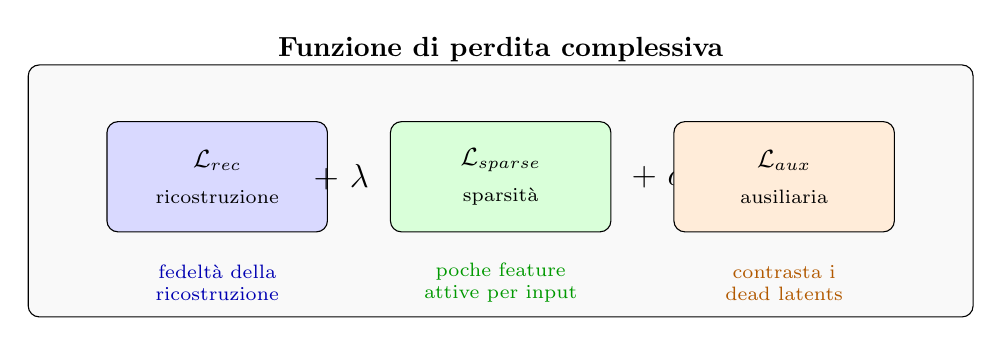
\begin{tikzpicture}[scale=0.9]
        % Box principale
        \node[draw, rectangle, minimum width=12cm, minimum height=3.2cm, fill=gray!5, rounded corners] at (0, 0) {};
        
        % Titolo
        \node[font=\bfseries] at (0, 2.0) {Funzione di perdita complessiva};
        
        % Tre componenti
        \node[draw, rectangle, minimum width=2.8cm, minimum height=1.4cm, fill=blue!15, rounded corners] (rec) at (-4, 0.2) {};
        \node[font=\small, align=center] at (-4, 0.2) {$\mathcal{L}_{\text{rec}}$\\[2pt]\scriptsize ricostruzione};
        
        \node[font=\large] at (-2.25, 0.2) {$+\ \lambda$};
        
        \node[draw, rectangle, minimum width=2.8cm, minimum height=1.4cm, fill=green!15, rounded corners] (sparse) at (0, 0.2) {};
        \node[font=\small, align=center] at (0, 0.2) {$\mathcal{L}_{\text{sparse}}$\\[2pt]\scriptsize sparsità};
        
        \node[font=\large] at (2.25, 0.2) {$+\ \alpha $ };
        
        \node[draw, rectangle, minimum width=2.8cm, minimum height=1.4cm, fill=orange!15, rounded corners] (aux) at (4, 0.2) {};
        \node[font=\small, align=center] at (4, 0.2) {$\mathcal{L}_{\text{aux}}$\\[2pt]\scriptsize ausiliaria};
        
        % Descrizioni sotto (più distanziate)
        \node[font=\scriptsize, align=center, blue!70!black] at (-4, -1.3) {fedeltà della\\ricostruzione};
        \node[font=\scriptsize, align=center, green!60!black] at (0, -1.3) {poche feature\\attive per input};
        \node[font=\scriptsize, align=center, orange!70!black] at (4, -1.3) {contrasta i\\dead latents};
        
    \end{tikzpicture}
    \caption{I tre componenti della funzione di perdita. La perdita di ricostruzione garantisce fedeltà semantica; il vincolo di sparsità forza rappresentazioni con poche attivazioni; la perdita ausiliaria previene il collasso di feature inutilizzate.}
    \label{fig:loss_components}
\end{figure}

Il bilanciamento tra questi termini è cruciale. Se $\lambda$ è troppo basso, il modello potrebbe attivare molte feature per ogni input, perdendo il vantaggio della sparsità. Se $\lambda$ è troppo alto, il modello potrebbe sacrificare la qualità della ricostruzione pur di mantenere poche attivazioni. O'Neill et al. osservano che, con l'approccio Top-K, il coefficiente $\lambda$ diventa meno critico perché la sparsità è imposta come vincolo rigido piuttosto che come penalità morbida. Il coefficiente $\alpha$ della perdita ausiliaria è tipicamente fissato a $1/32$, un valore che bilancia l'effetto di recupero dei dead latents senza interferire eccessivamente con l'obiettivo principale.
\subsubsection{Il vincolo di sparsità Top-K}
\label{subsubsec:topk_sparsity}

L'approccio tradizionale per indurre sparsità in un autoencoder è la regolarizzazione $L_1$: aggiungere alla loss un termine proporzionale alla somma delle attivazioni:
\begin{equation}
    \mathcal{L}_{\text{sparse}}^{L_1}(\mathbf{h}) = \sum_{i=1}^{n} |h_i|
\end{equation}
Questo termine penalizza le attivazioni non nulle, spingendo il modello a utilizzare poche feature. Tuttavia, la regolarizzazione $L_1$ presenta un problema noto come \textit{shrinkage}: per ridurre la penalità, il modello tende a sottostimare sistematicamente le attivazioni, producendo valori $h_i$ più bassi di quelli che sarebbero ottimali per la ricostruzione~\parencite{oneill2024disentangling}. Il risultato è una rappresentazione sì sparsa, ma anche meno fedele.

O'Neill et al. adottano un approccio diverso: il vincolo \textbf{Top-K} (o \textit{k-sparse})~\parencite{makhzani2013ksparse}. Invece di penalizzare le attivazioni con un termine morbido, si impone un vincolo rigido: per ogni input, solo le $k$ attivazioni più grandi vengono mantenute, mentre tutte le altre sono forzate a zero.

Formalmente, sia $\mathbf{z} = W_e \mathbf{x} + \mathbf{b}_e$ il vettore delle pre-attivazioni. Il vincolo Top-K opera in due passi:
\begin{enumerate}
    \item Si identificano gli indici delle $k$ componenti di $\mathbf{z}$ con valore più alto
    \item Si pongono a zero tutte le altre componenti
\end{enumerate}
L'attivazione finale è quindi:
\begin{equation}
    h_i = \begin{cases}
        \sigma(z_i) & \text{se } z_i \text{ è tra i } k \text{ valori più alti} \\
        0 & \text{altrimenti}
    \end{cases}
    \label{eq:topk_activation}
\end{equation}
dove $\sigma(\cdot)$ è la ReLU.

\begin{figure}[htbp]
    \centering
    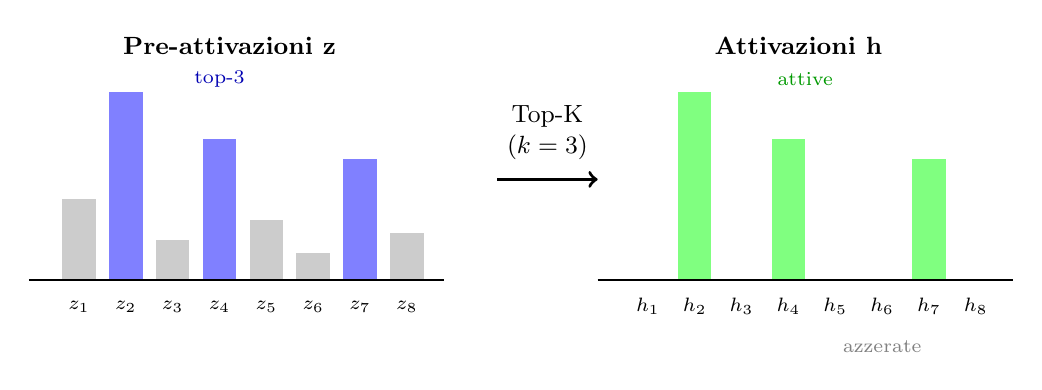
\begin{tikzpicture}[scale=0.85]
        
        % === Pre-attivazioni z ===
        \node[font=\small\bfseries] at (0, 3.5) {Pre-attivazioni $\mathbf{z}$};
        
        % Barre delle pre-attivazioni
        \fill[gray!40] (-2.5, 0) rectangle (-2.0, 1.2);
        \fill[blue!50] (-1.8, 0) rectangle (-1.3, 2.8);
        \fill[gray!40] (-1.1, 0) rectangle (-0.6, 0.6);
        \fill[blue!50] (-0.4, 0) rectangle (0.1, 2.1);
        \fill[gray!40] (0.3, 0) rectangle (0.8, 0.9);
        \fill[gray!40] (1.0, 0) rectangle (1.5, 0.4);
        \fill[blue!50] (1.7, 0) rectangle (2.2, 1.8);
        \fill[gray!40] (2.4, 0) rectangle (2.9, 0.7);
        
        % Asse
        \draw[thick] (-3, 0) -- (3.2, 0);
        
        % Labels
        \node[font=\scriptsize] at (-2.25, -0.4) {$z_1$};
        \node[font=\scriptsize] at (-1.55, -0.4) {$z_2$};
        \node[font=\scriptsize] at (-0.85, -0.4) {$z_3$};
        \node[font=\scriptsize] at (-0.15, -0.4) {$z_4$};
        \node[font=\scriptsize] at (0.55, -0.4) {$z_5$};
        \node[font=\scriptsize] at (1.25, -0.4) {$z_6$};
        \node[font=\scriptsize] at (1.95, -0.4) {$z_7$};
        \node[font=\scriptsize] at (2.65, -0.4) {$z_8$};
        
        % Freccia Top-K
        \draw[->, very thick] (4, 1.5) -- (5.5, 1.5);
        \node[font=\small, align=center] at (4.75, 2.2) {Top-K\\($k=3$)};
        
        % === Attivazioni h ===
        \node[font=\small\bfseries] at (8.5, 3.5) {Attivazioni $\mathbf{h}$};
        
        % Barre delle attivazioni (solo top-k)
        \fill[gray!20] (6.0, 0) rectangle (6.5, 0);
        \fill[green!50] (6.7, 0) rectangle (7.2, 2.8);
        \fill[gray!20] (7.4, 0) rectangle (7.9, 0);
        \fill[green!50] (8.1, 0) rectangle (8.6, 2.1);
        \fill[gray!20] (8.8, 0) rectangle (9.3, 0);
        \fill[gray!20] (9.5, 0) rectangle (10.0, 0);
        \fill[green!50] (10.2, 0) rectangle (10.7, 1.8);
        \fill[gray!20] (10.9, 0) rectangle (11.4, 0);
        
        % Asse
        \draw[thick] (5.5, 0) -- (11.7, 0);
        
        % Labels
        \node[font=\scriptsize] at (6.25, -0.4) {$h_1$};
        \node[font=\scriptsize] at (6.95, -0.4) {$h_2$};
        \node[font=\scriptsize] at (7.65, -0.4) {$h_3$};
        \node[font=\scriptsize] at (8.35, -0.4) {$h_4$};
        \node[font=\scriptsize] at (9.05, -0.4) {$h_5$};
        \node[font=\scriptsize] at (9.75, -0.4) {$h_6$};
        \node[font=\scriptsize] at (10.45, -0.4) {$h_7$};
        \node[font=\scriptsize] at (11.15, -0.4) {$h_8$};
        
        % Annotazioni
        \node[font=\scriptsize, blue!70!black] at (-0.15, 3.0) {top-3};
        \node[font=\scriptsize, green!60!black] at (8.6, 3.0) {attive};
        \node[font=\scriptsize, gray] at (9.75, -1.0) {azzerate};
        
    \end{tikzpicture}
    \caption{Il vincolo Top-K. A sinistra: le pre-attivazioni $\mathbf{z}$ calcolate dall'encoder. Le tre componenti con valore più alto sono evidenziate in blu. A destra: le attivazioni finali $\mathbf{h}$ dopo l'applicazione del vincolo Top-K con $k=3$. Solo le componenti selezionate (in verde) mantengono il loro valore; tutte le altre sono forzate a zero.}
    \label{fig:topk_mechanism}
\end{figure}

Il vantaggio del Top-K rispetto alla regolarizzazione $L_1$ è duplice. 

Il primo vantaggio è l'assenza di shrinkage. Le $k$ attivazioni selezionate mantengono il loro valore originale $\sigma(z_i)$, senza alcuna penalizzazione. Il modello può quindi apprendere attivazioni di intensità appropriata senza il compromesso imposto dalla regolarizzazione.

Il secondo vantaggio è il controllo diretto sulla sparsità. Con $L_1$, il livello di sparsità dipende dal coefficiente $\lambda$ e deve essere calibrato empiricamente. Con Top-K, la sparsità è deterministica: esattamente $k$ feature attive per input, né più né meno. Questo rende il comportamento del modello più prevedibile e i risultati più riproducibili.

La scelta del valore di $k$ è un iperparametro cruciale. Valori tipici variano tra 16 e 128, a seconda della complessità del dominio e della granularità desiderata~\parencite{oneill2024disentangling}. Un $k$ più basso produce rappresentazioni più sparse ma potenzialmente meno accurate; un $k$ più alto permette ricostruzioni migliori ma con meno separazione tra le feature. O'Neill et al. esplorano tre configurazioni principali:
\begin{itemize}
    \item \textbf{SAE16}: $k = 16$ attivazioni, $n = 2d = 3072$ feature totali
    \item \textbf{SAE32}: $k = 32$ attivazioni, $n = 4d = 6144$ feature totali
    \item \textbf{SAE64}: $k = 64$ attivazioni, $n = 6d = 9216$ feature totali
\end{itemize}
All'aumentare di $k$ e $n$, le feature apprese tendono a diventare più granulari e specifiche—un fenomeno che esploreremo nella Sezione~\ref{subsec:feature_splitting}.


\subsubsection{Auxiliary loss e il problema dei dead latents}
\label{subsubsec:auxiliary_loss}

Durante l'addestramento di uno Sparse Autoencoder può emergere un problema insidioso: alcune feature smettono di attivarsi completamente. Il vincolo Top-K seleziona, per ogni input, solo le $k$ attivazioni più alte; se una feature produce sistematicamente valori bassi, non verrà mai selezionata e i suoi parametri smetteranno di ricevere gradienti. Senza gradienti, la feature non può migliorare; senza miglioramento, continuerà a produrre valori bassi. Si innesca un circolo vizioso che porta la feature a ``morire''.

Queste feature inutilizzate sono chiamate \textbf{dead latents}. O'Neill et al.~\parencite{oneill2024disentangling} definiscono operativamente un latent come ``morto'' se non si è attivato per un'intera epoca di addestramento. Il problema non è solo teorico: nei primi esperimenti con SAE a $k=16$, gli autori osservano che una frazione significativa delle feature può diventare inattiva durante il training (Figura~\ref{fig:dead_latents}).

\begin{figure}[htbp]
    \centering
    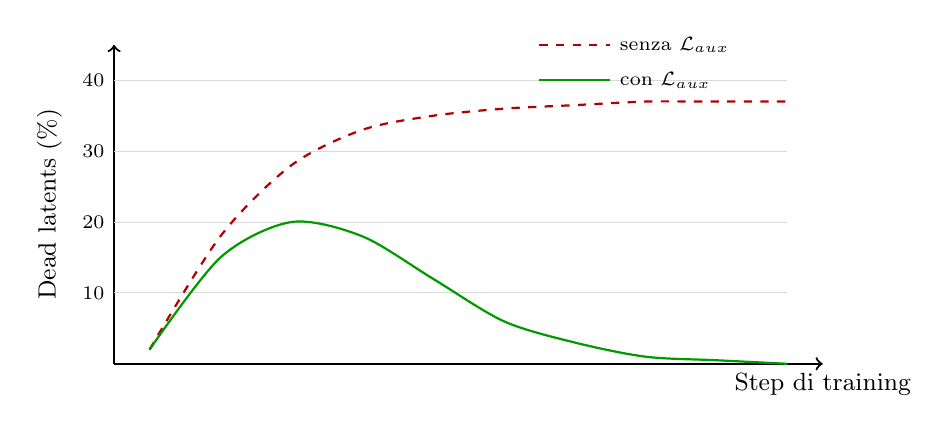
\begin{tikzpicture}[scale=0.9]
        % Asse x
        \draw[->, thick] (0, 0) -- (10, 0);
        \node[below, font=\small] at (10, 0) {Step di training};
        
        % Asse y
        \draw[->, thick] (0, 0) -- (0, 4.5);
        \node[above, rotate=90, font=\small] at (-0.6, 2.25) {Dead latents (\%)};
        
        % Griglia
        \draw[gray!30, thin] (0, 1) -- (9.5, 1);
        \draw[gray!30, thin] (0, 2) -- (9.5, 2);
        \draw[gray!30, thin] (0, 3) -- (9.5, 3);
        \draw[gray!30, thin] (0, 4) -- (9.5, 4);
        
        % Labels asse y
        \node[left, font=\scriptsize] at (0, 1) {10};
        \node[left, font=\scriptsize] at (0, 2) {20};
        \node[left, font=\scriptsize] at (0, 3) {30};
        \node[left, font=\scriptsize] at (0, 4) {40};
        
        % Curva (senza auxiliary loss)
        \draw[thick, red!70!black, dashed] plot[smooth] coordinates {
            (0.5, 0.2) (1.5, 1.8) (2.5, 2.8) (3.5, 3.3) (4.5, 3.5) (5.5, 3.6) (6.5, 3.65) (7.5, 3.7) (8.5, 3.7) (9.5, 3.7)
        };
        
        % Curva (con auxiliary loss)
        \draw[thick, green!60!black] plot[smooth] coordinates {
            (0.5, 0.2) (1.5, 1.5) (2.5, 2.0) (3.5, 1.8) (4.5, 1.2) (5.5, 0.6) (6.5, 0.3) (7.5, 0.1) (8.5, 0.05) (9.5, 0)
        };
        
        % Legenda
        \draw[thick, red!70!black, dashed] (6, 4.5) -- (7, 4.5);
        \node[right, font=\scriptsize] at (7, 4.5) {senza $\mathcal{L}_{\text{aux}}$};
        
        \draw[thick, green!60!black] (6, 4) -- (7, 4);
        \node[right, font=\scriptsize] at (7, 4) {con $\mathcal{L}_{\text{aux}}$};
        
    \end{tikzpicture}
    \caption{Evoluzione dei dead latents durante il training (illustrazione qualitativa basata sui risultati di O'Neill et al.). Senza la perdita ausiliaria, una frazione significativa di feature diventa permanentemente inattiva. Con la perdita ausiliaria, i dead latents vengono progressivamente ``rianimati'' fino a scomparire.}
    \label{fig:dead_latents}
\end{figure}
I dead latents rappresentano uno spreco di capacità. Se il modello ha $n = 3072$ feature ma 500 sono morte, la capacità effettiva si riduce a 2572 feature—vanificando parte del vantaggio dell'overcompletezza. Peggio ancora, le feature che sopravvivono potrebbero essere costrette a rappresentare più concetti di quanti ne potrebbero gestire, reintroducendo una forma di polisemantictà.
Per contrastare questo fenomeno, O'Neill et al. introducono una \textbf{perdita ausiliaria} ispirata alla tecnica dei ``ghost grads''~\parencite{jermyn2023ghostgrads}. L'idea è semplice: se una feature è morta, non riceve gradienti dalla loss principale perché non contribuisce alla ricostruzione. Ma possiamo \textit{forzarla} a contribuire chiedendole di ricostruire l'\textit{errore} del modello.
Formalmente, sia $\mathbf{e} = \mathbf{x} - \hat{\mathbf{x}}$ l'errore di ricostruzione del modello principale. La perdita ausiliaria chiede ai dead latents di modellare questo errore:
\begin{equation}
    \mathcal{L}_{\text{aux}}(\mathbf{x}, \hat{\mathbf{x}}) = \|\mathbf{e} - \hat{\mathbf{e}}\|_2^2
    \label{eq:auxiliary_loss}
\end{equation}
dove $\hat{\mathbf{e}} = W_d \mathbf{z}$ è la ricostruzione dell'errore ottenuta usando solo i dead latents. Il vettore $\mathbf{z}$ è una rappresentazione sparsa che utilizza esclusivamente le $k_{\text{aux}}$ feature attualmente inattive con le pre-attivazioni più alte.
Il meccanismo funziona così: le feature ``vive'' ricostruiscono $\mathbf{x}$ producendo $\hat{\mathbf{x}}$; le feature ``morte'' cercano di ricostruire l'errore residuo $\mathbf{e}$. Se un dead latent riesce a catturare parte dell'errore, la sua direzione $\mathbf{w}_i$ sta evidentemente codificando informazione utile che le feature attive non stanno rappresentando. Il gradiente della perdita ausiliaria ``risveglia'' questo latent, dandogli la possibilità di competere nuovamente per essere selezionato dal Top-K.
\begin{notebox}
\textbf{Il meccanismo della perdita ausiliaria}\\
\begin{enumerate}
    \item Le feature attive ricostruiscono l'input: $\hat{\mathbf{x}} = \sum_{i \in \text{attive}} h_i \mathbf{w}_i + \mathbf{b}_d$
    \item Si calcola l'errore residuo: $\mathbf{e} = \mathbf{x} - \hat{\mathbf{x}}$
    \item I dead latents cercano di ricostruire l'errore: $\hat{\mathbf{e}} = \sum_{j \in \text{morti}} z_j \mathbf{w}_j$
    \item Se ci riescono, ricevono gradienti e possono ``tornare in vita''
\end{enumerate}
\end{notebox}
Il parametro $k_{\text{aux}}$ controlla quanti dead latents vengono coinvolti in ogni step. O'Neill et al. utilizzano tipicamente $k_{\text{aux}} = 2k$: il doppio dei latenti attivi nel modello principale. Il coefficiente $\alpha$ nella loss complessiva (Equazione~\ref{eq:total_loss}) è fissato a $1/32$, un valore sufficientemente basso da non interferire con l'obiettivo principale di ricostruzione, ma abbastanza alto da garantire il recupero dei dead latents nel corso dell'addestramento.
L'efficacia di questa tecnica è notevole. O'Neill et al. riportano che, alla fine del training, tutti i modelli presentano zero dead latents—tutte le $n$ feature hanno imparato a contribuire alla rappresentazione. Questo risultato è particolarmente importante per l'interpretabilità: significa che l'intera capacità del modello è effettivamente utilizzata, e ogni direzione $\mathbf{w}_i$ nel decoder rappresenta potenzialmente un concetto distinto.
\subsection{Interpretabilità automatica delle feature}
\label{subsec:interpretability}
Lo Sparse Autoencoder produce una rappresentazione in cui ogni feature corrisponde a una direzione $\mathbf{w}_i$ nello spazio degli embedding e a un'attivazione $h_i$ che ne indica l'intensità. Ma una direzione geometrica, di per sé, non è interpretabile: per rendere le feature comprensibili agli esseri umani, dobbiamo associare a ciascuna un'etichetta semantica—un nome che descriva il concetto che quella feature cattura.
Un approccio manuale sarebbe impraticabile. Con migliaia di feature ($n = 3072$ o più), ispezionare una per una i testi che le attivano richiederebbe settimane di lavoro. O'Neill et al.~\parencite{oneill2024disentangling} propongono invece un approccio automatizzato: utilizzare un Large Language Model come \textbf{interprete} delle feature.
\subsubsection{L'Interpreter LLM}
\label{subsubsec:interpreter}
L'intuizione è semplice. Se una feature cattura un concetto semantico coerente, i testi che la attivano fortemente dovrebbero condividere qualcosa—un tema, un argomento, una proprietà stilistica. Un modello linguistico, esaminando questi testi, dovrebbe essere in grado di identificare il denominatore comune.
Il processo di interpretazione si articola in tre passi:
\textbf{Passo 1: Identificare i testi attivanti.} Per ogni feature $i$, si scorre l'intero corpus di documenti e si calcolano le attivazioni $h_i$ prodotte dall'encoder. Si selezionano i $k$ documenti con le attivazioni più alte—i testi che ``accendono'' maggiormente quella feature. Tipicamente $k = 5$.
\textbf{Passo 2: Identificare i contro-esempi.} Si selezionano anche alcuni documenti che \textit{non} attivano la feature ($h_i = 0$). Questi contro-esempi aiutano l'interprete a discriminare: il concetto cercato deve essere presente nei testi attivanti e assente nei contro-esempi.
\textbf{Passo 3: Interrogare l'LLM.} I testi attivanti e i contro-esempi vengono forniti a un modello linguistico insieme a un prompt che chiede di identificare il tema comune. L'LLM restituisce un'etichetta breve (1-8 parole) che descrive la feature.

\begin{figure}[htbp]
    \centering
    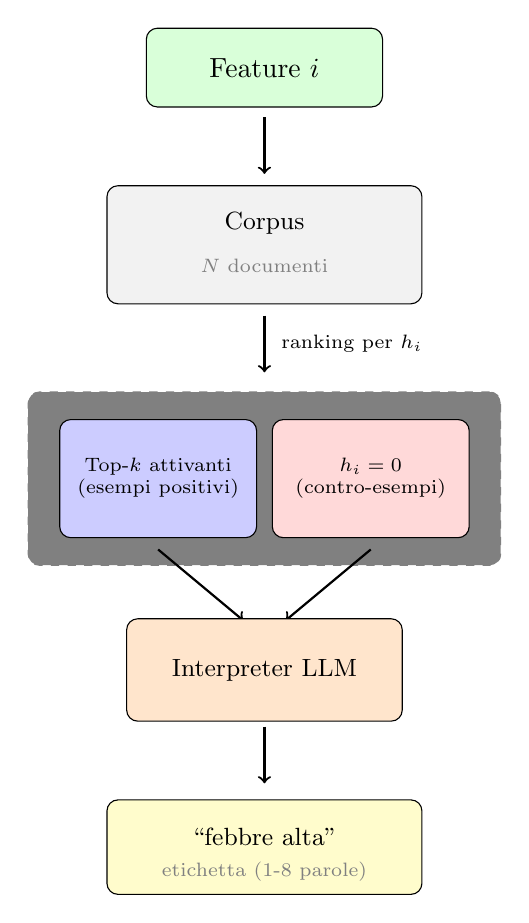
\begin{tikzpicture}[scale=0.9]
        
        % Feature box (top)
        \node[draw, rectangle, minimum width=3cm, minimum height=1cm, fill=green!15, rounded corners] (feature) at (0, 0) {Feature $i$};
        
        % Freccia verso corpus
        \draw[->, thick] (0, -0.7) -- (0, -1.5);
        
        % Corpus
        \node[draw, rectangle, minimum width=4cm, minimum height=1.5cm, fill=gray!10, rounded corners] (corpus) at (0, -2.5) {};
        \node[font=\small] at (0, -2.2) {Corpus};
        \node[font=\scriptsize, gray] at (0, -2.8) {$N$ documenti};
        
        % Freccia verso selezione
        \draw[->, thick] (0, -3.5) -- (0, -4.3);
        \node[right, font=\scriptsize] at (0.1, -3.9) {ranking per $h_i$};
        
        % Box contenitore per esempi
        \node[draw, rectangle, minimum width=6cm, minimum height=2.2cm, fill=white, rounded corners, dashed, gray] at (0, -5.8) {};
        
        % Testi attivanti (sinistra)
        \node[draw, rectangle, minimum width=2.5cm, minimum height=1.5cm, fill=blue!20, rounded corners] (pos) at (-1.5, -5.8) {};
        \node[font=\scriptsize, align=center] at (-1.5, -5.8) {Top-$k$ attivanti\\(esempi positivi)};
        
        % Testi non attivanti (destra)
        \node[draw, rectangle, minimum width=2.5cm, minimum height=1.5cm, fill=red!15, rounded corners] (neg) at (1.5, -5.8) {};
        \node[font=\scriptsize, align=center] at (1.5, -5.8) {$h_i = 0$\\(contro-esempi)};
        
        % Frecce verso LLM
        \draw[->, thick] (-1.5, -6.8) -- (-0.3, -7.8);
        \draw[->, thick] (1.5, -6.8) -- (0.3, -7.8);
        
        % LLM
        \node[draw, rectangle, minimum width=3.5cm, minimum height=1.3cm, fill=orange!20, rounded corners] (llm) at (0, -8.5) {};
        \node[font=\small, align=center] at (0, -8.5) {Interpreter LLM};
        
        % Freccia verso output
        \draw[->, thick] (0, -9.3) -- (0, -10.1);
        
        % Output
        \node[draw, rectangle, minimum width=4cm, minimum height=1.2cm, fill=yellow!20, rounded corners] (label) at (0, -11) {};
        \node[font=\small, align=center] at (0, -10.85) {``febbre alta''};
        \node[font=\scriptsize, gray] at (0, -11.35) {etichetta (1-8 parole)};
        
    \end{tikzpicture}
    \caption{Il processo di interpretazione automatica. Per ogni feature, si identificano i testi che la attivano maggiormente e quelli che non la attivano affatto. Un LLM esamina entrambi gli insiemi e produce un'etichetta che descrive il concetto catturato dalla feature.}
    \label{fig:interpreter_process}
\end{figure}

Il prompt fornito all'interprete è progettato con cura. O'Neill et al. istruiscono il modello a comportarsi come un ``meticoloso ricercatore'' che deve scoprire quale comportamento attiva un certo neurone. Il prompt richiede di:
\begin{enumerate}
    \item Elencare i potenziali temi comuni tra i testi attivanti, a diversi livelli di granularità
    \item Escludere i temi presenti anche nei contro-esempi
    \item Applicare il rasoio di Occam: scegliere la spiegazione più semplice compatibile con i dati
    \item Formulare l'etichetta finale in 1-8 parole
\end{enumerate}
Il riferimento al rasoio di Occam è particolarmente importante. Senza questa indicazione, l'interprete potrebbe produrre etichette troppo specifiche (che catturano solo un sottoinsieme dei testi attivanti) o troppo generiche (che non discriminano dai contro-esempi). La richiesta di semplicità guida verso etichette al giusto livello di astrazione.
\subsubsection{Implementazione in PRISMA}
\label{subsubsec:prisma_interpreter}
In PRISMA, l'interpretazione delle feature è implementata attraverso l'integrazione con Ollama, un framework per l'esecuzione locale di modelli linguistici. Questa scelta presenta vantaggi significativi: non richiede connessione a servizi cloud, garantisce la privacy dei dati (particolarmente importante nel contesto medico), e permette di processare grandi volumi di feature senza costi di API.
Il processo segue fedelmente lo schema descritto sopra. Per ogni feature del SAE addestrato:
\begin{enumerate}
    \item Il modulo \texttt{explorer} scansiona tutti i documenti del corpus
    \item Identifica i documenti con le attivazioni più alte per quella feature
    \item Seleziona documenti con attivazione nulla come contro-esempi
    \item Costruisce il prompt con esempi positivi e negativi
    \item Invia la richiesta al modello locale via Ollama
    \item Memorizza l'etichetta risultante nel database
\end{enumerate}

Il prompt utilizzato in PRISMA è adattato al dominio medico-pediatrico. L'LLM viene istruito a cercare concetti clinici specifici—sintomi, diagnosi, trattamenti, fasce d'età—piuttosto che temi generici. Questa specializzazione migliora la qualità delle etichette nel dominio di applicazione.

\begin{notebox}
\textbf{Esempio di interpretazione}\\
Supponiamo che una feature si attivi fortemente sui seguenti testi:
\begin{itemize}
    \item ``Paziente presenta temperatura corporea 39.2°C''
    \item ``Febbre persistente da tre giorni, non responsiva a paracetamolo''
    \item ``Iperpiressia in paziente pediatrico di 4 anni''
\end{itemize}
E non si attivi su:
\begin{itemize}
    \item ``Esame obiettivo nella norma, paziente apiretico''
    \item ``Tosse secca senza rialzo termico''
\end{itemize}
L'interprete, confrontando i due insiemi, identificherebbe il tema comune e produrrebbe l'etichetta: ``febbre / iperpiressia''.
\end{notebox}

È importante sottolineare i limiti di questo approccio. L'interpretazione automatica è un'euristica, non una dimostrazione formale che la feature catturi esattamente il concetto indicato dall'etichetta. Alcune feature potrebbero essere polisemantiche (catturare più concetti correlati), altre potrebbero essere difficili da descrivere in poche parole. O'Neill et al. propongono un secondo passo—un \textit{Predictor} LLM che valida le etichette predicendo le attivazioni su testi unseen—ma questa validazione formale esula dagli scopi dell'implementazione attuale di PRISMA. Le etichette vanno quindi intese come ipotesi interpretative da verificare qualitativamente, non come verità assolute.

\subsection{Feature Families: struttura gerarchica dei concetti}
\label{subsec:feature_families}
Finora abbiamo trattato le feature come entità indipendenti: ogni $\mathbf{w}_i$ rappresenta un concetto, ogni $h_i$ ne indica l'intensità. Ma l'analisi empirica delle feature apprese rivela una struttura più ricca: le feature non sono isolate, ma si organizzano spontaneamente in \textbf{famiglie gerarchiche}—gruppi di concetti correlati che spaziano da temi generali a sotto-temi specifici.
\subsubsection{Co-attivazione e struttura emergente}
\label{subsubsec:coactivation}
L'osservazione di partenza è semplice: alcune feature tendono ad attivarsi insieme. Se un testo parla di ``ottimizzazione in reti neurali'', è probabile che attivi simultaneamente feature legate a ``gradient descent'', ``learning rate'', ``Adam optimizer''. Questa co-attivazione non è casuale—riflette relazioni semantiche reali tra i concetti.
O'Neill et al.~\parencite{oneill2024disentangling} quantificano questo fenomeno attraverso la \textbf{matrice di co-occorrenza} $C$. Per ogni coppia di feature $(i, j)$, si conta quante volte entrambe sono attive sullo stesso documento:
\begin{equation}
    C_{ij} = \sum_{k=1}^{N} A_{ik} \cdot A_{jk}
    \label{eq:cooccurrence}
\end{equation}
dove $A_{ik} = 1$ se la feature $i$ è attiva sul documento $k$, e $A_{ik} = 0$ altrimenti. La matrice $C$ è simmetrica: $C_{ij} = C_{ji}$.
Per rendere i valori comparabili tra feature con frequenze diverse, si normalizza per la frequenza di attivazione:
\begin{equation}
    C_{ij}^{\text{norm}} = \frac{C_{ij}}{f_i + \epsilon}
    \label{eq:cooccurrence_norm}
\end{equation}
dove $f_i = \sum_k A_{ik}$ è la frequenza di attivazione della feature $i$ e $\epsilon$ è una piccola costante per la stabilità numerica.
Analizzando questa matrice emerge un pattern caratteristico: esistono gruppi di feature con alta co-occorrenza interna e bassa co-occorrenza con l'esterno. Ma la struttura non è simmetrica all'interno dei gruppi. Tipicamente, una feature—il \textbf{parent}—co-occorre con tutte le altre del gruppo, mentre le altre—i \textbf{children}—co-occorrono col parent ma raramente tra loro.


\begin{figure}[htbp]
    \centering
    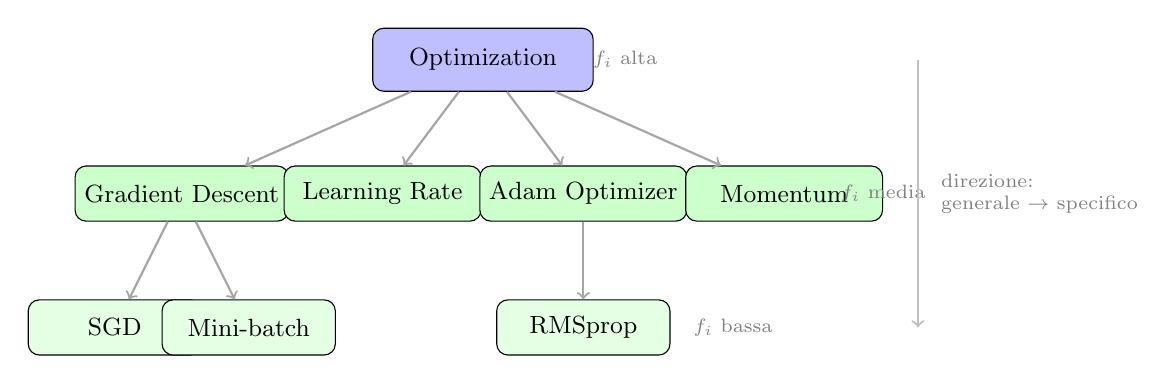
\begin{tikzpicture}[
        scale=0.85,
        every node/.style={font=\small},
        parent/.style={draw, rectangle, rounded corners, fill=blue!25, minimum width=2.8cm, minimum height=0.8cm},
        child/.style={draw, rectangle, rounded corners, fill=green!20, minimum width=2.5cm, minimum height=0.7cm},
        arrow/.style={->, thick, gray!70}
    ]
        
        % Parent (root)
        \node[parent] (root) at (0, 0) {Optimization};
        
        % Children (livello 1)
        \node[child] (c1) at (-4.5, -2) {Gradient Descent};
        \node[child] (c2) at (-1.5, -2) {Learning Rate};
        \node[child] (c3) at (1.5, -2) {Adam Optimizer};
        \node[child] (c4) at (4.5, -2) {Momentum};
        
        % Grandchildren (livello 2) - solo per alcuni
        \node[child, fill=green!10, minimum width=2.2cm] (gc1) at (-5.5, -4) {SGD};
        \node[child, fill=green!10, minimum width=2.2cm] (gc2) at (-3.5, -4) {Mini-batch};
        \node[child, fill=green!10, minimum width=2.2cm] (gc3) at (1.5, -4) {RMSprop};
        
        % Archi
        \draw[arrow] (root) -- (c1);
        \draw[arrow] (root) -- (c2);
        \draw[arrow] (root) -- (c3);
        \draw[arrow] (root) -- (c4);
        \draw[arrow] (c1) -- (gc1);
        \draw[arrow] (c1) -- (gc2);
        \draw[arrow] (c3) -- (gc3);
        
        % Annotazioni densità
        \node[right, font=\scriptsize, gray] at (1.5, 0) {$f_i$ alta};
        \node[right, font=\scriptsize, gray] at (5.2, -2) {$f_i$ media};
        \node[right, font=\scriptsize, gray] at (3, -4) {$f_i$ bassa};
        
        % Freccia indicante direzione
        \draw[->, thick, gray!50] (6.5, 0) -- (6.5, -4);
        \node[right, font=\scriptsize, gray, align=left] at (6.7, -2) {direzione:\\generale $\to$ specifico};
        
    \end{tikzpicture}
    \caption{Esempio di feature family nel dominio del machine learning (adattato da O'Neill et al.). La radice ``Optimization'' è il parent: un concetto generale con alta densità di attivazione $f_i$. Gli archi sono orientati verso feature con densità decrescente, riflettendo la gerarchia semantica dal generale allo specifico.}
    \label{fig:feature_family_tree}
\end{figure}

\subsubsection{Identificazione delle famiglie}
\label{subsubsec:family_identification}

Per estrarre automaticamente le feature families dalla matrice di co-occorrenza, O'Neill et al. sviluppano un algoritmo basato su grafi. L'intuizione è costruire un albero che colleghi le feature più correlate, poi interpretare le relazioni padre-figlio in base alla frequenza di attivazione. L'algoritmo procede come segue:

\begin{enumerate}
    \item \textbf{Selezione delle feature.} Si considerano solo le feature altamente interpretabili, definite da O'Neill et al. come quelle con $\text{F1} \geq 0.8$ e correlazione di Pearson $\geq 0.8$ nel task di predizione dell'Interpreter. Questa selezione preliminare garantisce che le famiglie estratte siano composte da feature semanticamente significative.
    
    \item \textbf{Costruzione del grafo pesato.} Si parte dalla matrice di co-occorrenza normalizzata $C^{\text{norm}}$ e si applica una \textbf{soglia} $\tau$ per filtrare le relazioni deboli. Due feature $i$ e $j$ vengono collegate da un arco se e solo se:
    \begin{equation}
        C^{\text{norm}}_{ij} > \tau
        \label{eq:threshold}
    \end{equation}
    dove tipicamente $\tau = 0.1$. L'intuizione è semplice: se la feature $j$ si attiva in meno del 10\% dei casi in cui si attiva la feature $i$, la relazione è troppo debole per essere considerata significativa. Il risultato è un grafo pesato $G = (V, E)$ in cui i nodi $V$ sono le feature e gli archi $E$ collegano coppie con co-occorrenza sopra soglia, con peso $w_{ij} = C^{\text{norm}}_{ij}$.
    
    \item \textbf{Estrazione del Maximum Spanning Tree.} Dal grafo pesato $G$ si estrae il \textbf{Maximum Spanning Tree} (MST)—l'albero di copertura che connette tutti i nodi massimizzando la somma dei pesi degli archi. A differenza del più noto Minimum Spanning Tree usato per trovare connessioni a costo minimo, qui si vuole preservare le relazioni \textit{più forti}. L'MST ha due proprietà: (1) connette tutte le feature in un'unica struttura, e (2) evita i cicli, garantendo una topologia ad albero che si presta naturalmente all'interpretazione gerarchica. In pratica, l'MST seleziona, per ogni feature, la connessione più forte con il resto della struttura, scartando le ridondanze.
    
    \item \textbf{Orientamento degli archi.} L'albero ottenuto è inizialmente non diretto. Per convertirlo in una gerarchia, si assegna una direzione a ogni arco basandosi sulla \textbf{densità di attivazione} $f_i = \sum_k A_{ik}$, ovvero il numero totale di documenti su cui la feature $i$ si attiva. Gli archi vengono orientati \textit{dalla feature più densa verso quella meno densa}:
    \begin{equation}
        i \to j \quad \text{se} \quad f_i > f_j
        \label{eq:edge_direction}
    \end{equation}
    L'intuizione semantica è che i concetti generali si attivano più frequentemente dei concetti specifici: ``ottimizzazione'' compare in più paper di ``Adam optimizer'', ``malattie respiratorie'' in più referti di ``polmonite da Pneumocystis''. Dopo l'orientamento, l'albero diventa un grafo diretto aciclico (DAG) con una chiara direzione dal generale allo specifico.
    
    \item \textbf{Identificazione delle radici e estrazione delle famiglie.} Nel grafo diretto, le \textbf{radici} sono i nodi senza archi entranti—feature che non sono ``figlie'' di nessun'altra feature nel grafo. Ogni radice rappresenta il concetto più generale di una potenziale famiglia. A partire da ciascuna radice, si esplora l'albero con una visita in profondità (\textit{depth-first search}), raccogliendo tutti i discendenti. L'insieme formato dalla radice (il \textbf{parent}) e dai suoi discendenti (i \textbf{children}) costituisce una feature family. Se l'albero ha più componenti connesse dopo il thresholding, si ottengono più famiglie indipendenti.
    
    
\end{enumerate}

\subsection{Feature Splitting: granularità emergente}
\label{subsec:feature_splitting}

La capacità di un SAE—determinata dal numero di latenti totali $n$ e dal numero di latenti attivi $k$—non influenza solo la qualità della ricostruzione, ma anche la \textit{granularità} delle feature apprese. All'aumentare della capacità, i concetti rappresentati diventano progressivamente più specifici: una feature che in un SAE piccolo cattura ``ottimizzazione'' può \textit{scindersi} in un SAE più grande in feature distinte per ``gradient descent'', ``Adam'', ``learning rate scheduling''. Questo fenomeno, chiamato \textbf{feature splitting}, rivela come la struttura semantica emerga gradualmente con l'aumentare delle risorse rappresentazionali.

\subsubsection{Il fenomeno dello splitting}
\label{subsubsec:splitting_phenomenon}

L'osservazione di partenza è empirica: addestrando SAE con capacità crescenti sullo stesso corpus, alcune feature si ``dividono'' in sotto-feature più specifiche. O'Neill et al. studiano questo fenomeno confrontando sistematicamente SAE di dimensioni diverse—in particolare SAE16 ($k=16$, $n=3072$), SAE32 ($k=32$, $n=6144$) e SAE64 ($k=64$, $n=9216$).

Per tracciare come le feature evolvono tra modelli, si utilizza un approccio basato sul \textbf{nearest neighbour}. Data una coppia di SAE con $n_1$ e $n_2$ feature rispettivamente, si calcola una matrice di similarità $S \in \mathbb{R}^{n_1 \times n_2}$ dove ogni elemento è la similarità del coseno tra i vettori decoder:
\begin{equation}
    S_{ij} = \frac{\mathbf{w}_i^T \mathbf{w}_j}{\|\mathbf{w}_i\| \|\mathbf{w}_j\|}
    \label{eq:feature_similarity}
\end{equation}
dove $\mathbf{w}_i$ è il vettore decoder della feature $i$ nel SAE più piccolo e $\mathbf{w}_j$ quello della feature $j$ nel SAE più grande. Per ogni feature nel SAE grande, si identifica la feature più simile nel SAE piccolo—il suo ``nearest neighbour''.

L'analisi rivela un pattern consistente: all'aumentare di $k$ e $n$, la similarità massima tra nearest neighbour \textit{diminuisce}. In altre parole, le feature dei SAE più grandi sono progressivamente più distanti da quelle dei SAE più piccoli. Questo indica che i modelli con maggiore capacità apprendono rappresentazioni più fini e specializzate.

\begin{figure}[htbp]
    \centering
    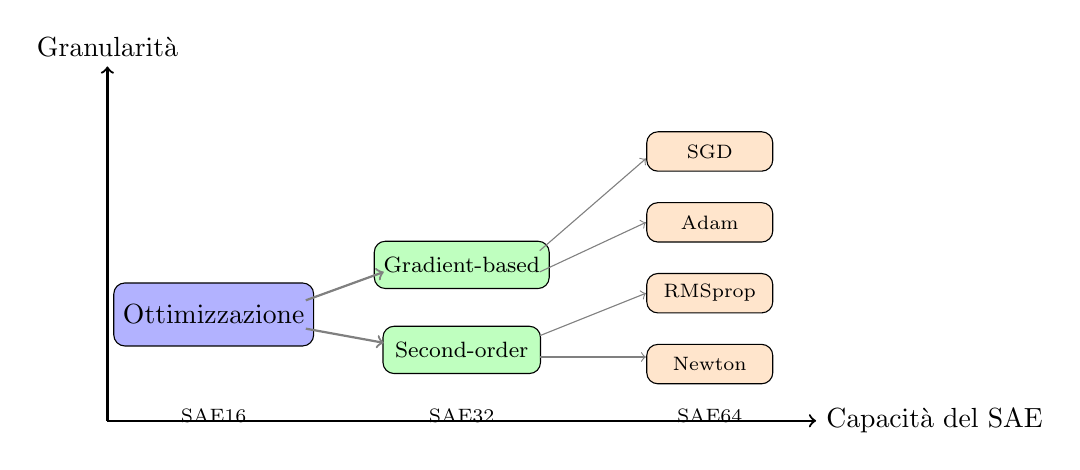
\begin{tikzpicture}[scale=0.9]
        % Assi
        \draw[->, thick] (0, 0) -- (10, 0) node[right] {Capacità del SAE};
        \draw[->, thick] (0, 0) -- (0, 5) node[above] {Granularità};
        
        % SAE16
        \node[draw, rectangle, rounded corners, fill=blue!30, minimum width=2.5cm, minimum height=0.8cm] (sae16) at (1.5, 1.5) {Ottimizzazione};
        \node[below, font=\scriptsize] at (1.5, 0.3) {SAE16};
        
        % SAE32 - splitting in 2
        \node[draw, rectangle, rounded corners, fill=green!25, minimum width=2cm, minimum height=0.6cm, font=\footnotesize] (sae32a) at (5, 2.2) {Gradient-based};
        \node[draw, rectangle, rounded corners, fill=green!25, minimum width=2cm, minimum height=0.6cm, font=\footnotesize] (sae32b) at (5, 1) {Second-order};
        \node[below, font=\scriptsize] at (5, 0.3) {SAE32};
        
        % SAE64 - splitting in 4
        \node[draw, rectangle, rounded corners, fill=orange!20, minimum width=1.6cm, minimum height=0.5cm, font=\scriptsize] (sae64a) at (8.5, 3.8) {SGD};
        \node[draw, rectangle, rounded corners, fill=orange!20, minimum width=1.6cm, minimum height=0.5cm, font=\scriptsize] (sae64b) at (8.5, 2.8) {Adam};
        \node[draw, rectangle, rounded corners, fill=orange!20, minimum width=1.6cm, minimum height=0.5cm, font=\scriptsize] (sae64c) at (8.5, 1.8) {RMSprop};
        \node[draw, rectangle, rounded corners, fill=orange!20, minimum width=1.6cm, minimum height=0.5cm, font=\scriptsize] (sae64d) at (8.5, 0.8) {Newton};
        \node[below, font=\scriptsize] at (8.5, 0.3) {SAE64};
        
        % Frecce di splitting
        \draw[->, gray, thick] (2.8, 1.7) -- (3.9, 2.1);
        \draw[->, gray, thick] (2.8, 1.3) -- (3.9, 1.1);
        
        \draw[->, gray] (6.1, 2.4) -- (7.6, 3.7);
        \draw[->, gray] (6.1, 2.1) -- (7.6, 2.8);
        \draw[->, gray] (6.1, 1.2) -- (7.6, 1.8);
        \draw[->, gray] (6.1, 0.9) -- (7.6, 0.9);
        
    \end{tikzpicture}
    \caption{Illustrazione del feature splitting. Una feature generale in un SAE piccolo (``Ottimizzazione'') si scinde progressivamente in feature più specifiche all'aumentare della capacità. SAE32 distingue metodi gradient-based da metodi del secondo ordine; SAE64 arriva a distinguere singoli algoritmi.}
    \label{fig:feature_splitting}
\end{figure}

\subsubsection{Feature ricorrenti e feature nuove}
\label{subsubsec:recurrent_novel}

Non tutte le feature si comportano allo stesso modo al variare della capacità. O'Neill et al. identificano due categorie distinte:

Le \textbf{feature ricorrenti} appaiono con alta similarità ($S_{ij} > 0.95$) in SAE di dimensioni diverse. Queste feature rappresentano concetti ``atomici'' che non si scompongono ulteriormente—ad esempio, ``O-type stars'' in astrofisica o ``Generative Adversarial Networks'' in machine learning. La loro stabilità attraverso modelli di capacità diversa suggerisce che corrispondono a concetti fondamentali del dominio, non ulteriormente scomponibili.

Le \textbf{feature nuove} (o \textit{novel features}) hanno invece bassa similarità con qualsiasi feature del SAE più piccolo. Queste emergono solo quando la capacità è sufficiente a rappresentarle separatamente. Un SAE piccolo potrebbe non avere abbastanza dimensioni per distinguere ``polmonite batterica'' da ``polmonite virale'', rappresentandole con un'unica feature ``polmonite''. Un SAE più grande può permettersi questa distinzione, facendo emergere feature nuove che non hanno un corrispondente diretto nel modello più piccolo.

\begin{notebox}
\textbf{Splitting vs.\ feature nuove}\\[0.5em]
È importante distinguere tra:
\begin{itemize}
    \item \textbf{Feature splitting}: una feature del SAE piccolo si ``divide'' in più feature correlate nel SAE grande. Le nuove feature hanno alta similarità di attivazione con la feature originale su un sottoinsieme dei documenti.
    \item \textbf{Feature nuove}: feature nel SAE grande che non hanno corrispondenti semantici nel SAE piccolo. Possono emergere perché il SAE piccolo non aveva capacità sufficiente per rappresentare quel concetto, oppure perché aggregava concetti non correlati.
\end{itemize}
La distinzione si basa sia sulla similarità geometrica ($S_{ij}$) che sulla similarità di attivazione sui documenti.
\end{notebox}

\subsubsection{Implicazioni per la dimensionalità delle rappresentazioni}
\label{subsubsec:dimensionality_implications}

Il feature splitting ha implicazioni profonde per comprendere la struttura delle rappresentazioni apprese. L'esistenza di feature ricorrenti suggerisce che esiste un ``nucleo'' di concetti stabili che qualsiasi SAE sufficientemente capace deve rappresentare. L'emergere di feature nuove indica invece che la capacità aggiuntiva viene utilizzata per raffinare la granularità della rappresentazione.

Questa osservazione solleva una domanda fondamentale: \textit{quante} feature sono realmente necessarie per rappresentare un dominio? E quante di queste feature vengono effettivamente utilizzate dal modello?

La risposta non è semplicemente $n$ (il numero totale di latenti) né $k$ (il numero di latenti attivi per input). La \textbf{dimensionalità effettiva} della rappresentazione dipende da come le feature vengono utilizzate \textit{nel loro insieme} attraverso il corpus. Se molte feature sono altamente correlate nei loro pattern di attivazione—come accade nelle feature families—la dimensionalità effettiva può essere significativamente inferiore al numero nominale di feature.

Questa intuizione motiva l'analisi della \textbf{matrice di attivazione sparsa} $A \in \mathbb{R}^{N \times n}$, dove $N$ è il numero di documenti e $n$ il numero di feature. Ogni riga $A_k$ contiene le attivazioni $h_i$ per il documento $k$. La struttura di questa matrice—in particolare il suo \textbf{rango effettivo}—rivela quanto della capacità teorica del SAE viene realmente sfruttata e come le feature si organizzano in strutture di correlazione. Questa analisi sarà oggetto del Capitolo~\ref{chap:results}, dove utilizzeremo metriche come l'\textit{Effective Rank} per quantificare la dimensionalità intrinseca delle rappresentazioni sparse apprese da PRISMA.

\begin{figure}[htbp]
    \centering
    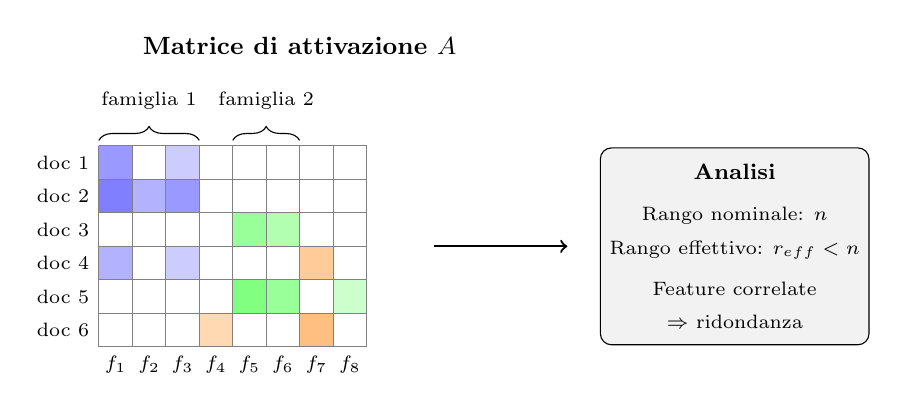
\begin{tikzpicture}[scale=0.85]
        
        % Matrice di attivazione
        \node[font=\small\bfseries] at (3, 4.5) {Matrice di attivazione $A$};
        
        % Griglia matrice
        \def\rows{6}
        \def\cols{8}
        \def\cellsize{0.5}
        
        % Sfondo celle con pattern di sparsità
        % Documento 1: feature 1, 3 attive
        \fill[blue!40] (0*\cellsize, 5*\cellsize) rectangle (1*\cellsize, 6*\cellsize);
        \fill[blue!20] (2*\cellsize, 5*\cellsize) rectangle (3*\cellsize, 6*\cellsize);
        
        % Documento 2: feature 1, 2, 3 attive (correlate)
        \fill[blue!50] (0*\cellsize, 4*\cellsize) rectangle (1*\cellsize, 5*\cellsize);
        \fill[blue!30] (1*\cellsize, 4*\cellsize) rectangle (2*\cellsize, 5*\cellsize);
        \fill[blue!40] (2*\cellsize, 4*\cellsize) rectangle (3*\cellsize, 5*\cellsize);
        
        % Documento 3: feature 5, 6 attive
        \fill[green!40] (4*\cellsize, 3*\cellsize) rectangle (5*\cellsize, 4*\cellsize);
        \fill[green!30] (5*\cellsize, 3*\cellsize) rectangle (6*\cellsize, 4*\cellsize);
        
        % Documento 4: feature 1, 3, 7 attive
        \fill[blue!30] (0*\cellsize, 2*\cellsize) rectangle (1*\cellsize, 3*\cellsize);
        \fill[blue!20] (2*\cellsize, 2*\cellsize) rectangle (3*\cellsize, 3*\cellsize);
        \fill[orange!40] (6*\cellsize, 2*\cellsize) rectangle (7*\cellsize, 3*\cellsize);
        
        % Documento 5: feature 5, 6, 8 attive
        \fill[green!50] (4*\cellsize, 1*\cellsize) rectangle (5*\cellsize, 2*\cellsize);
        \fill[green!40] (5*\cellsize, 1*\cellsize) rectangle (6*\cellsize, 2*\cellsize);
        \fill[green!20] (7*\cellsize, 1*\cellsize) rectangle (8*\cellsize, 2*\cellsize);
        
        % Documento 6: feature 4, 7 attive
        \fill[orange!30] (3*\cellsize, 0*\cellsize) rectangle (4*\cellsize, 1*\cellsize);
        \fill[orange!50] (6*\cellsize, 0*\cellsize) rectangle (7*\cellsize, 1*\cellsize);
        
        % Griglia
        \draw[gray, thin] (0, 0) grid[step=\cellsize] (\cols*\cellsize, \rows*\cellsize);
        
        % Labels
        \node[left, font=\scriptsize] at (0, 5.5*\cellsize) {doc 1};
        \node[left, font=\scriptsize] at (0, 4.5*\cellsize) {doc 2};
        \node[left, font=\scriptsize] at (0, 3.5*\cellsize) {doc 3};
        \node[left, font=\scriptsize] at (0, 2.5*\cellsize) {doc 4};
        \node[left, font=\scriptsize] at (0, 1.5*\cellsize) {doc 5};
        \node[left, font=\scriptsize] at (0, 0.5*\cellsize) {doc 6};
        
        \node[below, font=\scriptsize] at (0.5*\cellsize, 0) {$f_1$};
        \node[below, font=\scriptsize] at (1.5*\cellsize, 0) {$f_2$};
        \node[below, font=\scriptsize] at (2.5*\cellsize, 0) {$f_3$};
        \node[below, font=\scriptsize] at (3.5*\cellsize, 0) {$f_4$};
        \node[below, font=\scriptsize] at (4.5*\cellsize, 0) {$f_5$};
        \node[below, font=\scriptsize] at (5.5*\cellsize, 0) {$f_6$};
        \node[below, font=\scriptsize] at (6.5*\cellsize, 0) {$f_7$};
        \node[below, font=\scriptsize] at (7.5*\cellsize, 0) {$f_8$};
        
        % Annotazioni
        \draw[decorate, decoration={brace, amplitude=5pt, raise=2pt}] 
            (0, 6*\cellsize) -- (3*\cellsize, 6*\cellsize);
        \node[above, font=\scriptsize] at (1.5*\cellsize, 6*\cellsize + 0.4) {famiglia 1};
        
        \draw[decorate, decoration={brace, amplitude=5pt, raise=2pt}] 
            (4*\cellsize, 6*\cellsize) -- (6*\cellsize, 6*\cellsize);
        \node[above, font=\scriptsize] at (5*\cellsize, 6*\cellsize + 0.4) {famiglia 2};
        
        % Freccia verso analisi
        \draw[->, thick] (5, 1.5) -- (7, 1.5);
        
        % Box analisi
        \node[draw, rectangle, rounded corners, fill=gray!10, minimum width=3cm, minimum height=2.5cm, align=center] at (9.5, 1.5) {
            \footnotesize\textbf{Analisi}\\[0.3em]
            \scriptsize Rango nominale: $n$\\
            \scriptsize Rango effettivo: $r_{\text{eff}} < n$\\[0.3em]
            \scriptsize Feature correlate\\
            \scriptsize $\Rightarrow$ ridondanza
        };
        
    \end{tikzpicture}
    \caption{La matrice di attivazione sparsa $A$ rivela la struttura delle rappresentazioni. Feature che tendono ad attivarsi insieme (colori simili) formano gruppi correlati. Il rango effettivo della matrice è inferiore al numero nominale di feature, riflettendo la ridondanza introdotta dalle feature families e dallo splitting.}
    \label{fig:activation_matrix}
\end{figure}